\documentclass[11pt]{article}
\usepackage[top=2cm,left=2cm,right=2cm,bottom=2cm]{geometry}
\usepackage[doublespacing]{setspace}
\usepackage{graphicx}
\usepackage{xcolor}
\usepackage{subfigure}
\usepackage[hidelinks]{hyperref}
\usepackage{amsmath}
\usepackage{amssymb}
\usepackage{lscape}
\usepackage{booktabs}
\usepackage[localise]{xepersian}
\settextfont{XB Niloofar}


\begin{document}
	\شروع{وسط‌چین}
	به نام خدا\\
	\vspace{1cm}
	\begin{figure}[h]
		\begin{center}
			\includegraphics[width=0.3\linewidth]{"D:/Logo/UT"}
		\end{center}
	\end{figure}
	{\درشت‌درشت دانشکده مهندسی مکانیک}\\
	\vspace{1cm}
	{\بزرگ \سیاه{نام درس: هوش مصنوعی}}\\
	
	\vspace{0.5cm}
	{\درشت‌درشت تمرین ۳(شبکه عصبی)}
	\vspace{1.5cm}
	
	\vspace{1.5cm}
	{\درشت‌درشت {\سیاه استاد درس:} دکتر شریعت‌پناهی}\\
	\vspace{2cm}
	{\درشت‌درشت {\سیاه دانشجو:}}\\
	{\درشت مهدی نوذری\\
	810601139}\\
	\vspace{3cm}
	بهار ۱۴۰۳\\
	\پایان{وسط‌چین}
	\pagebreak
		تمامی فایل‌ها در \lr{Github} موجود هستند:
	\href{https://github.com/Morphit/UT_AI_1403}{\lr{https://github.com/Morphit/UT\_AI\_1403}}
	\section{شبکه \lr{MLP}}
	داده‌های در اختیار ما برای این مسئله شامل اطلاعات تصاویر ۲۸ در ۲۸ به صورت پیکسلی است که هر پیکسل یک مقدار از ۰ تا ۲۵۵ را داراست و نشان‌دهنده آن پیکسل در طیف خاکستری است. برچسب داده‌ها نیز شامل یک عدد از ۱ تا ۲۴ است که به معنای حروف A تا Y باشد.\\
	ابتدا ۷ عدد از این داده‌ها را به صورت تصادفی جدا کرده و آن‌ها را رسم می‌کنیم. این کار در 
	\autoref{fig:random_samples}
	نشان داده شده است.\\
	ساختار شبکه \lr{MLP} استفاده شده در 
	\autoref{fig:MLP_structure} 
	آمده است. این شبکه از دو لایه پنهان \lr{Dense} و یک لایه \lr{Dropout} به منظور کم کردن احتمال اورفیت شدن بهره می‌برد. توابع فعال‌سازی لایه‌های پنهان \lr{Relu} می‌باشد و تابع لایه خروجی \lr{Softmax} است. علت انتخاب تابع \lr{Softmax} برای خروجی این است که در لایه خروجی به تعداد کلاس‌ها نورون وجود دارد که هرکدام یک مقدار را خروجی می‌دهند. این تابع بیشترین مقدار خروجی‌ها را به ۱ و سایر را به ۰ تبدیل می‌کند که نهایتا به معنی انتخاب یک کلاس و انجام دسته‌بندی است.
	\begin{figure}[!h]
		\centerline{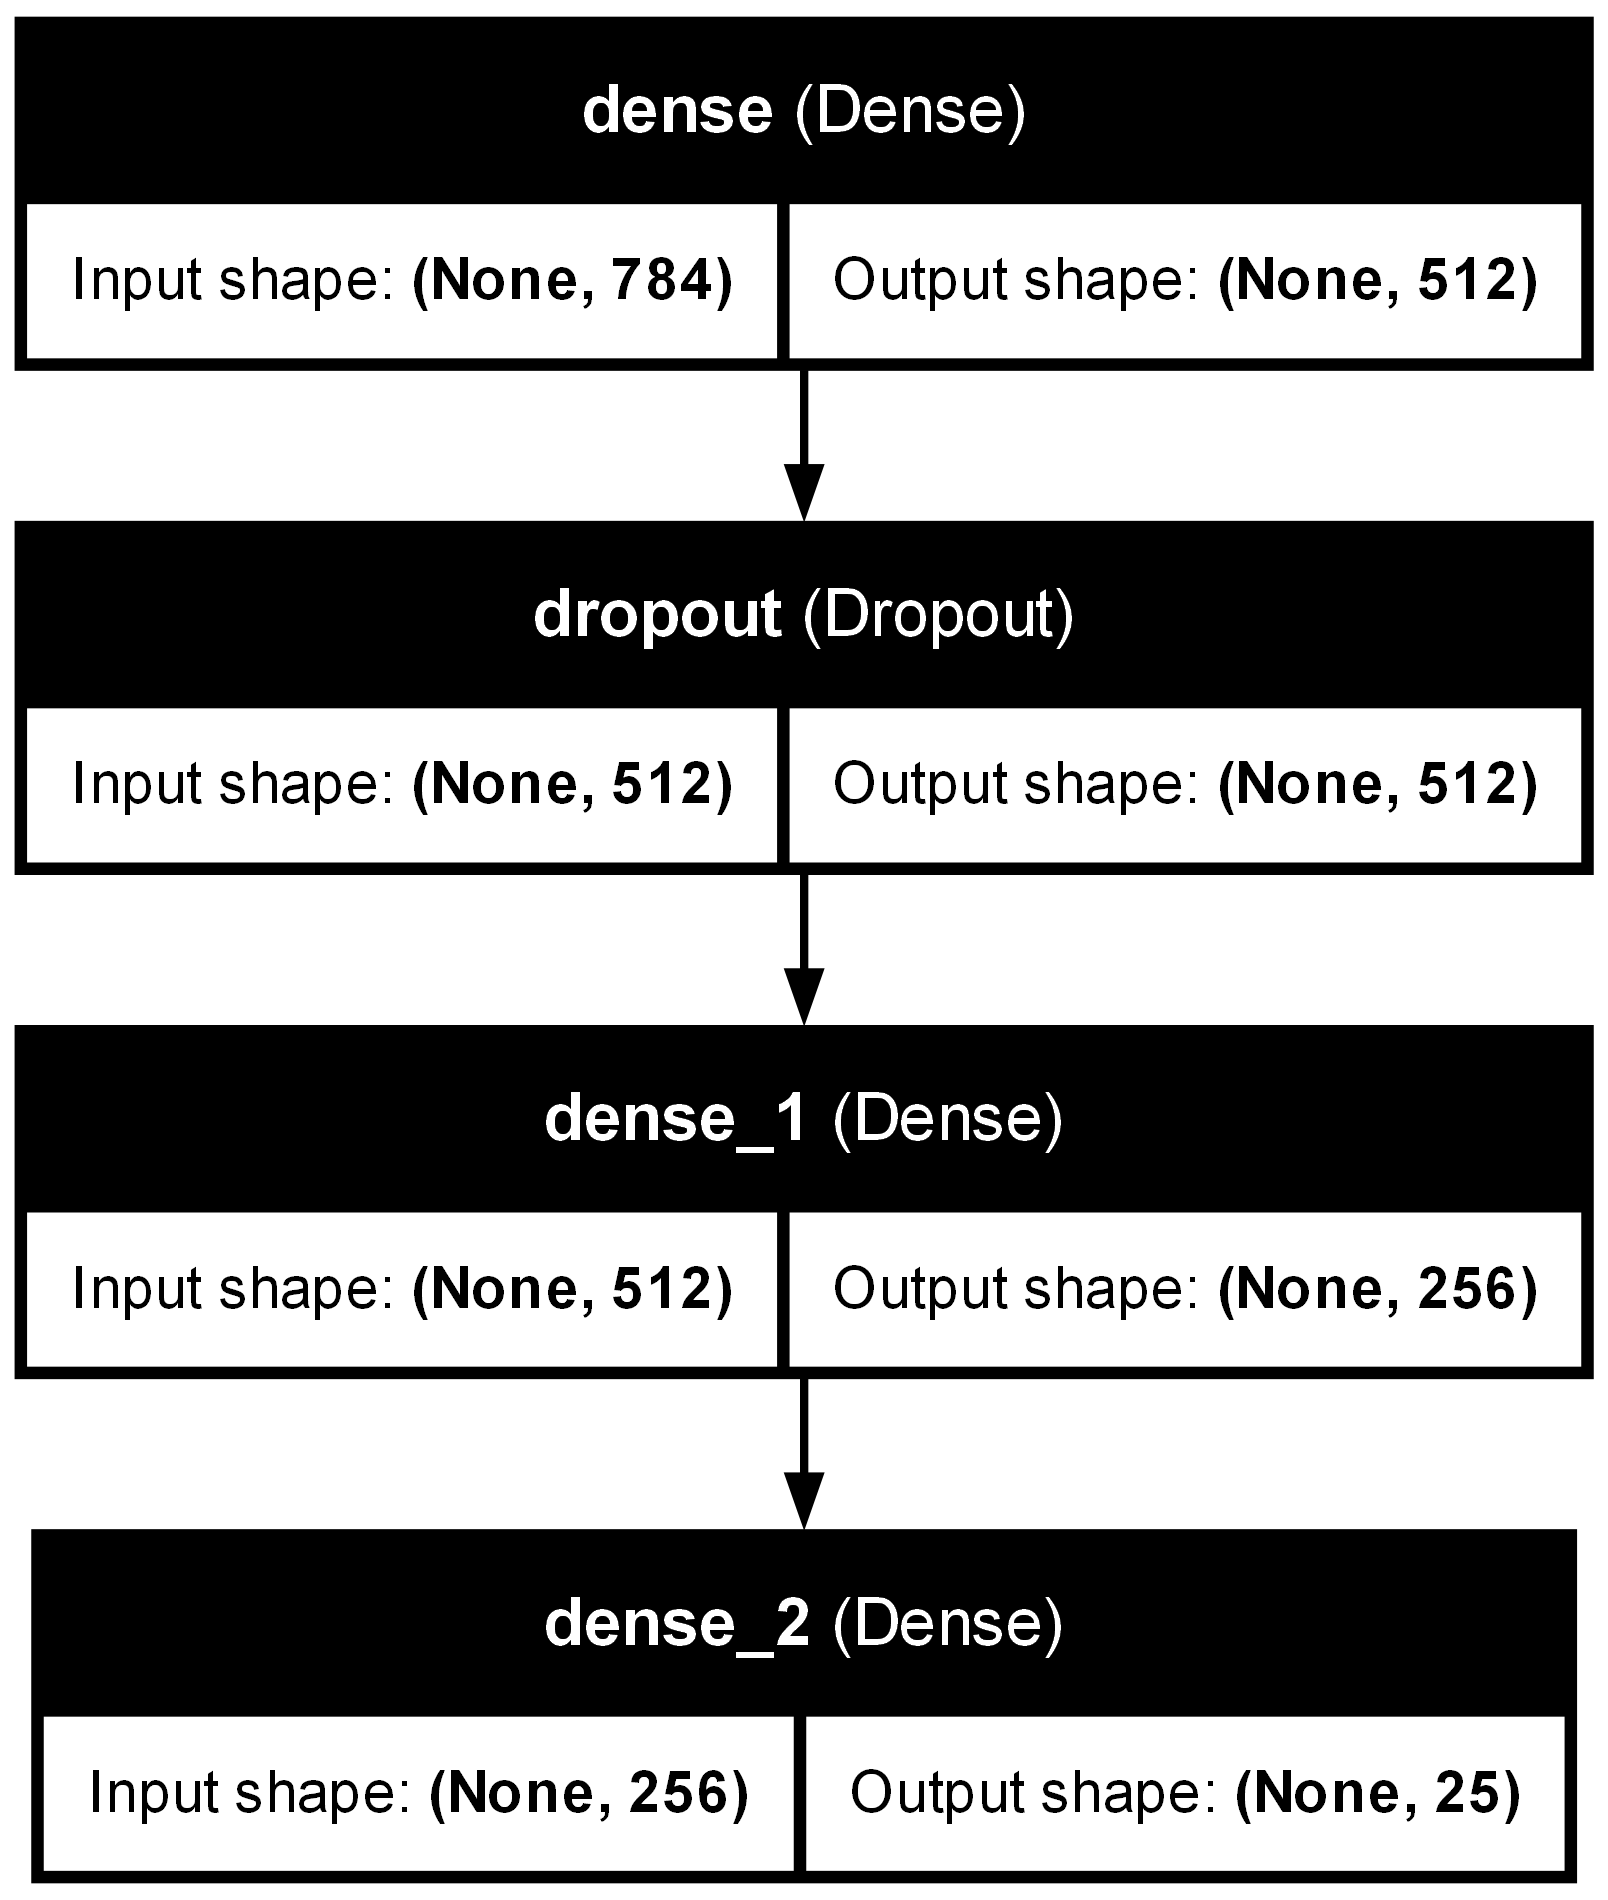
\includegraphics[width=0.5\linewidth]{../HW3_1/model_structure.png}}
		\caption{}
		\label{fig:MLP_structure}
	\end{figure}\\
		\begin{figure*}[!h]
		\centering
		\subfigure[]{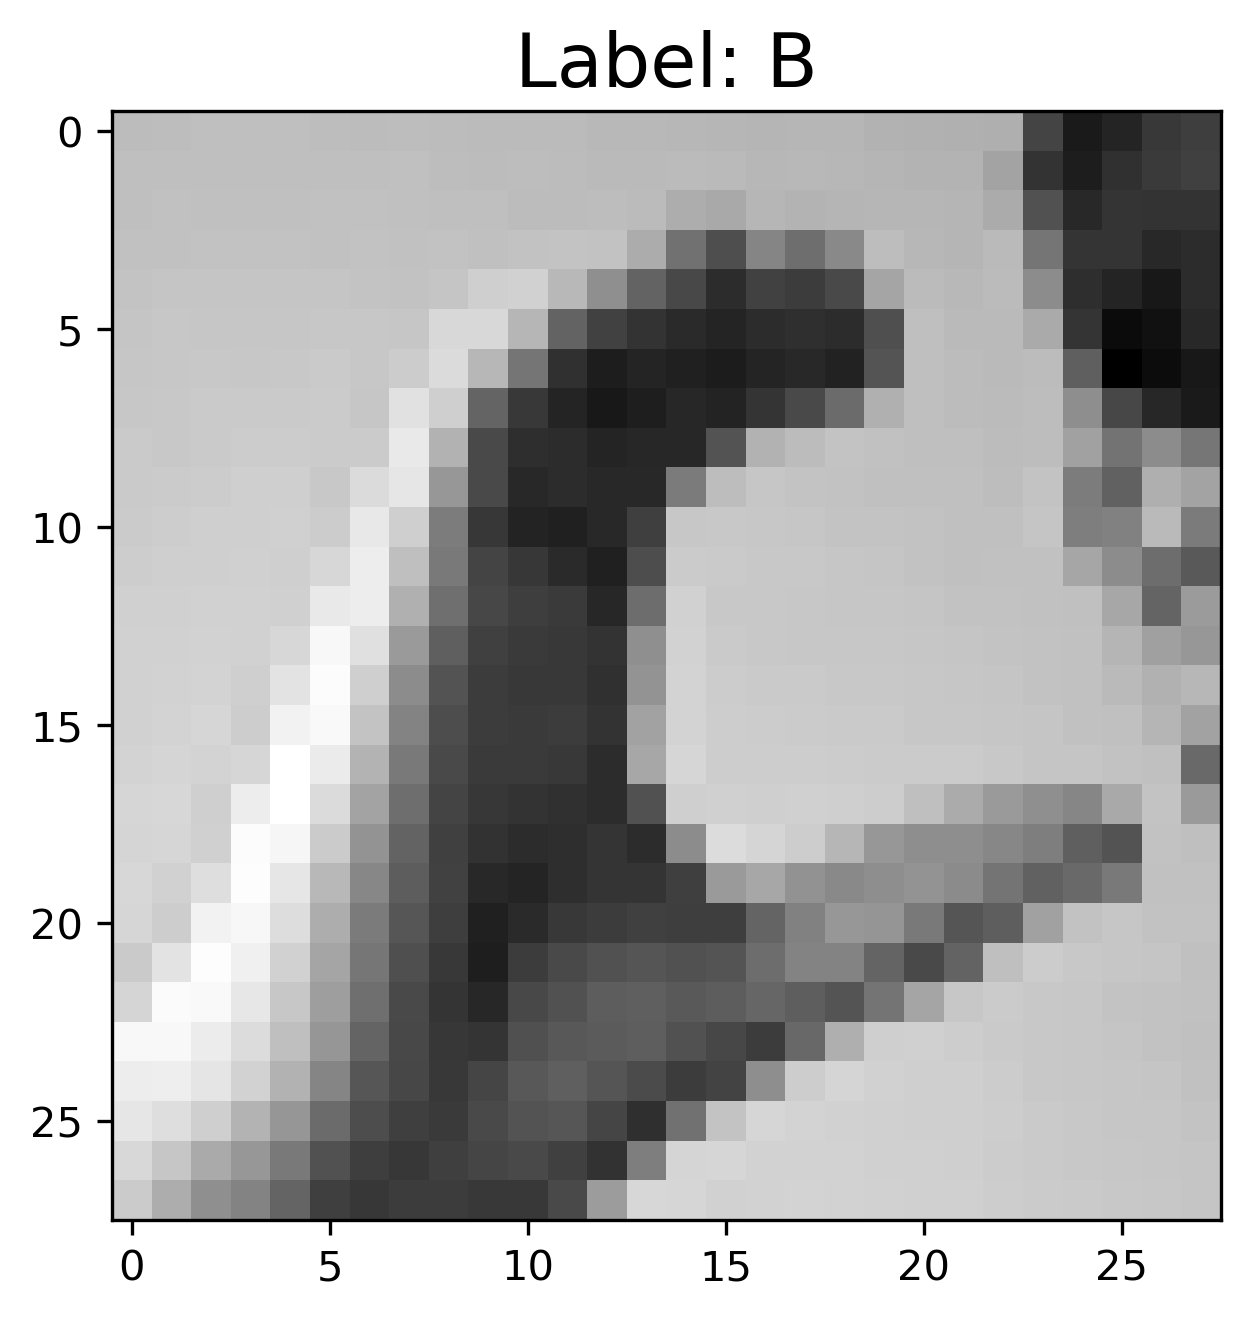
\includegraphics[height=0.31\linewidth]{../HW3_1/Sample1.png}}
		\subfigure[]{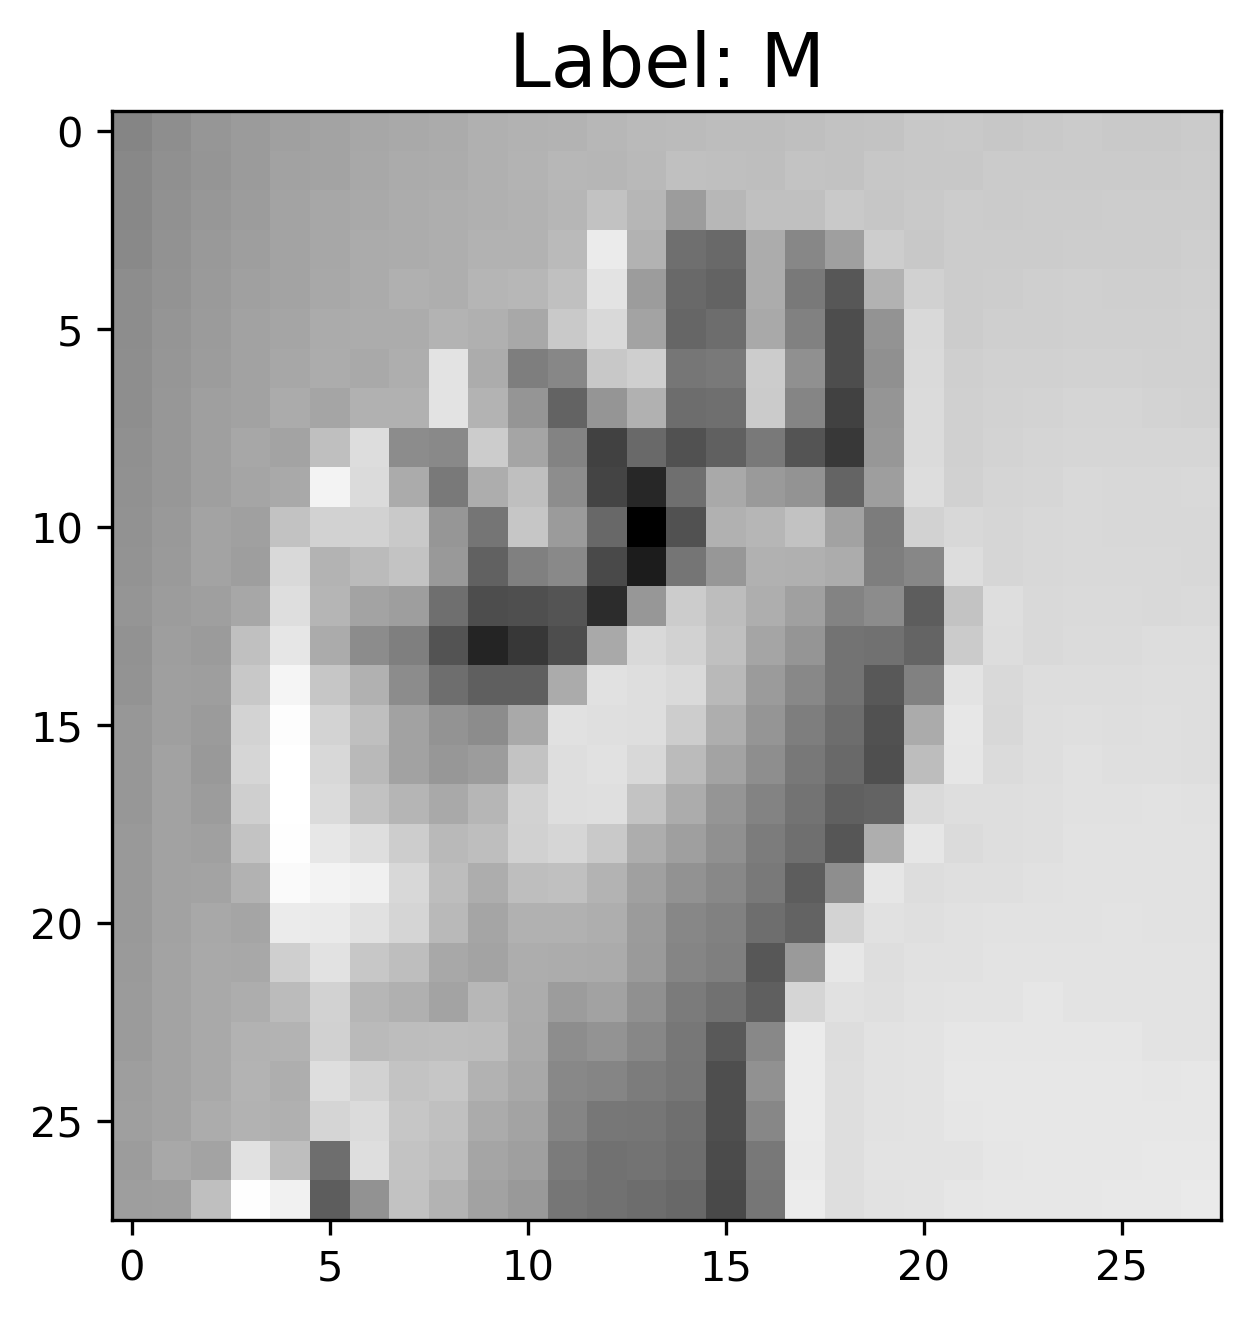
\includegraphics[height=0.31\linewidth]{../HW3_1/Sample2.png}}
		\subfigure[]{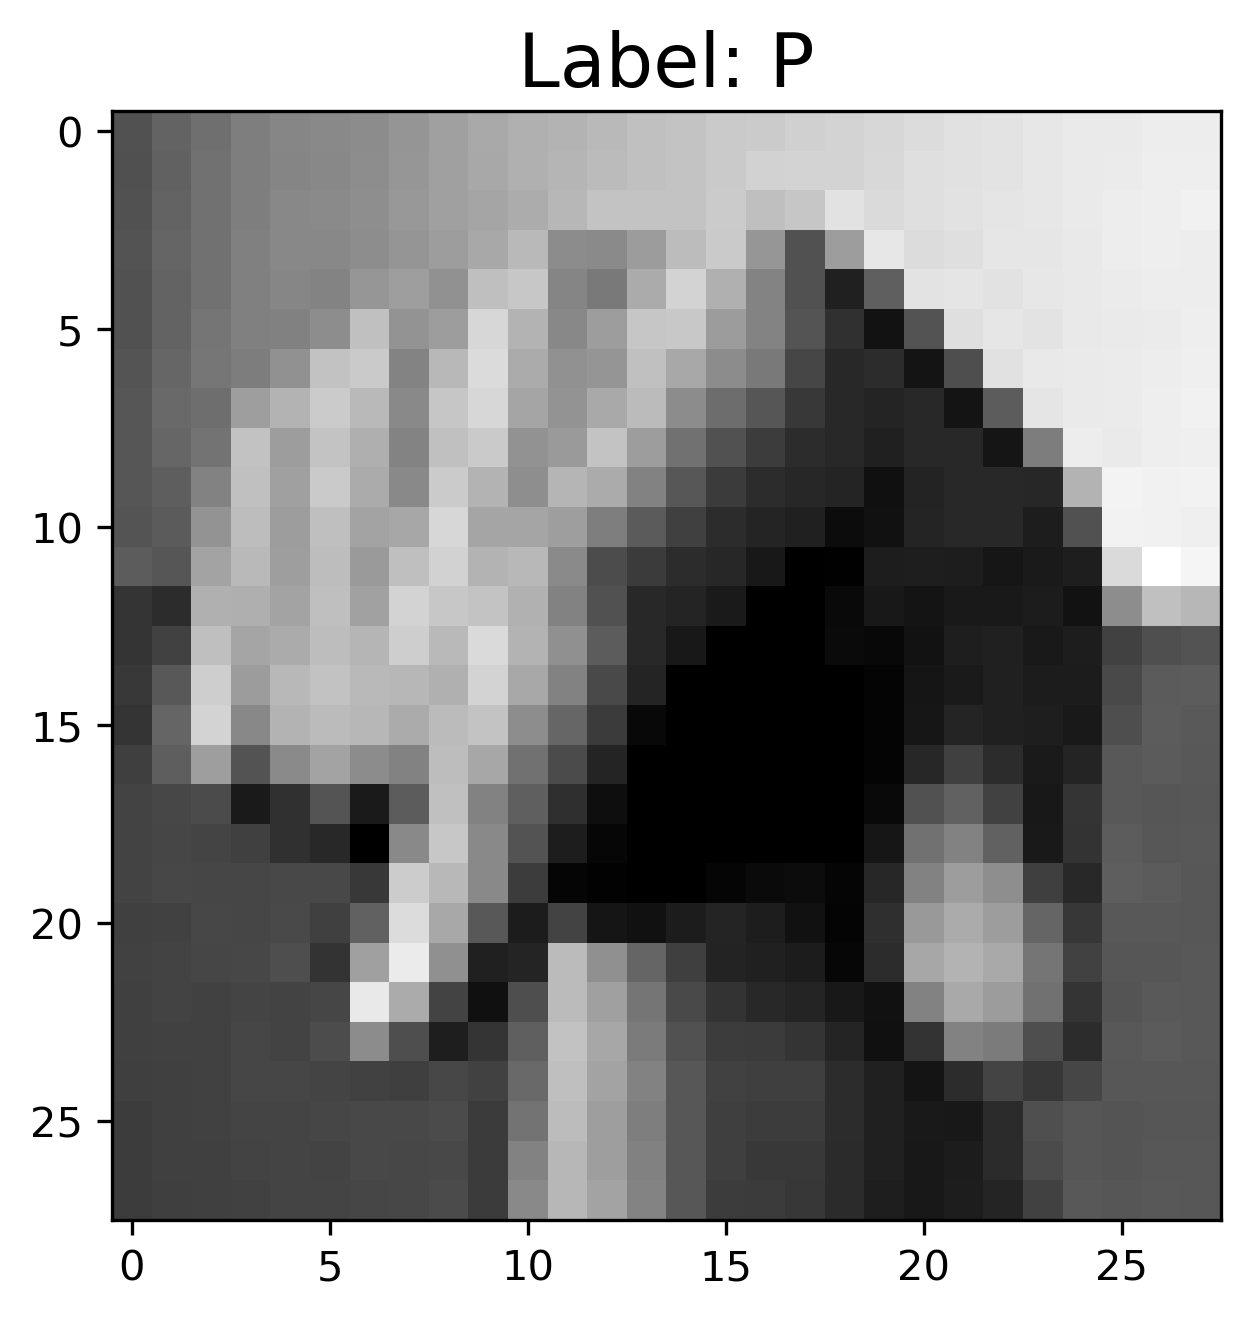
\includegraphics[height=0.31\linewidth]{../HW3_1/Sample3.png}}
		\subfigure[]{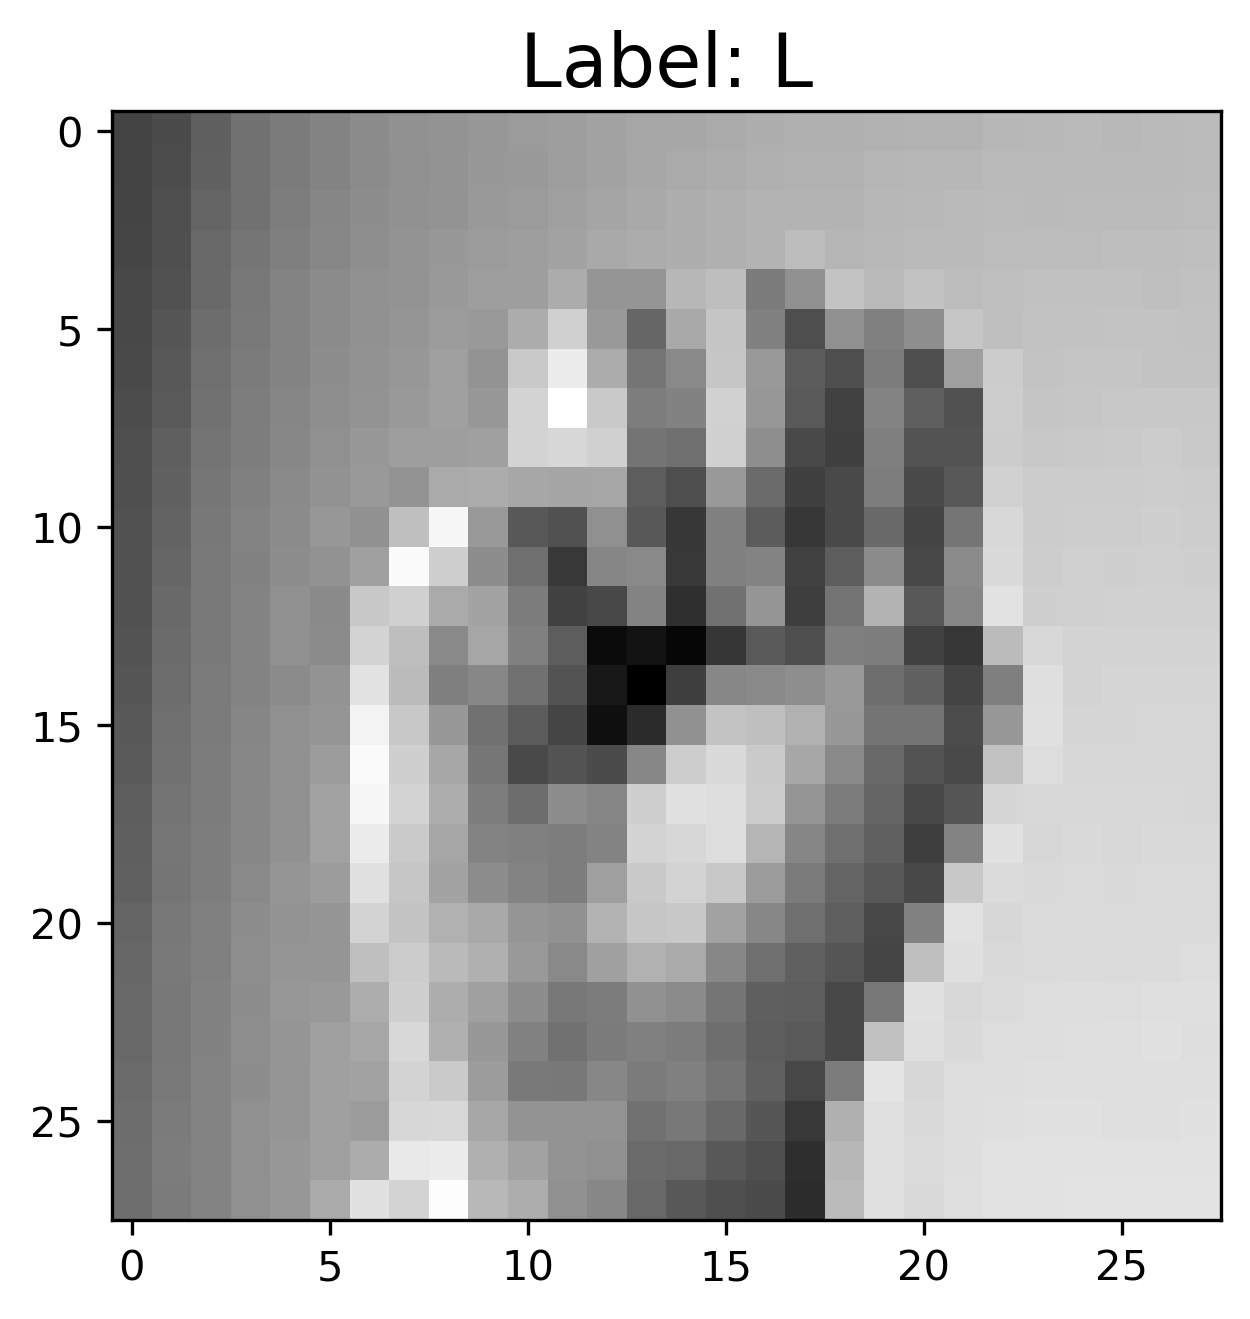
\includegraphics[height=0.31\linewidth]{../HW3_1/Sample4.png}}
		\subfigure[]{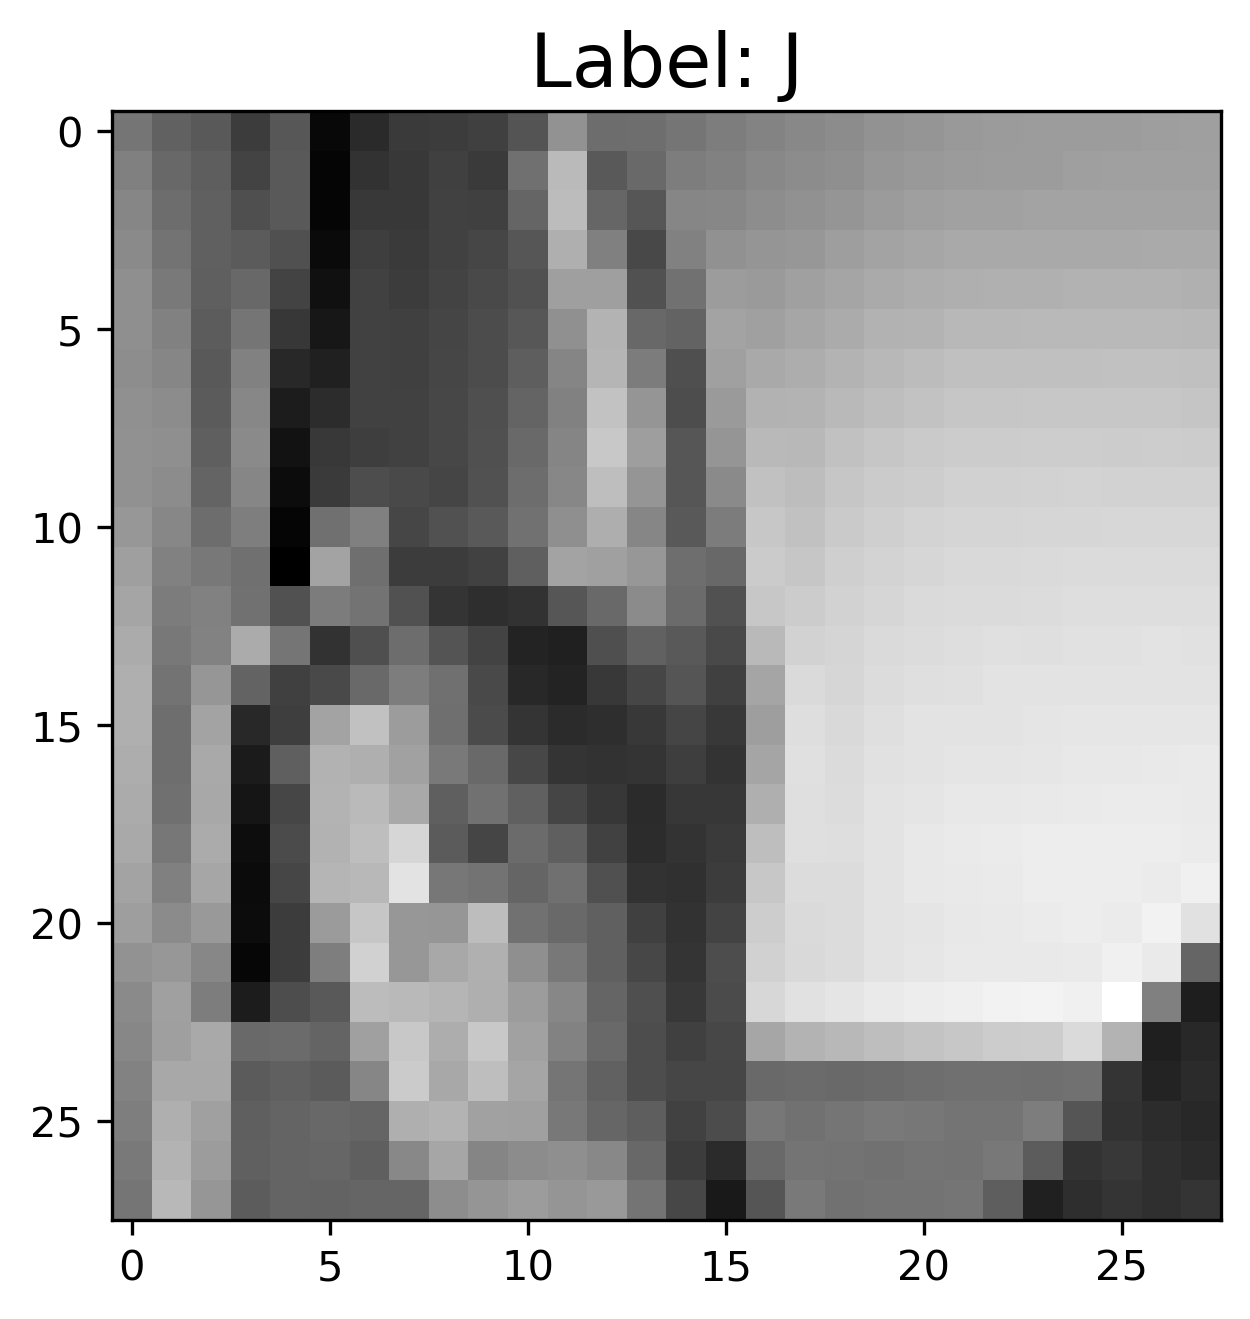
\includegraphics[height=0.31\linewidth]{../HW3_1/Sample5.png}}
		\subfigure[]{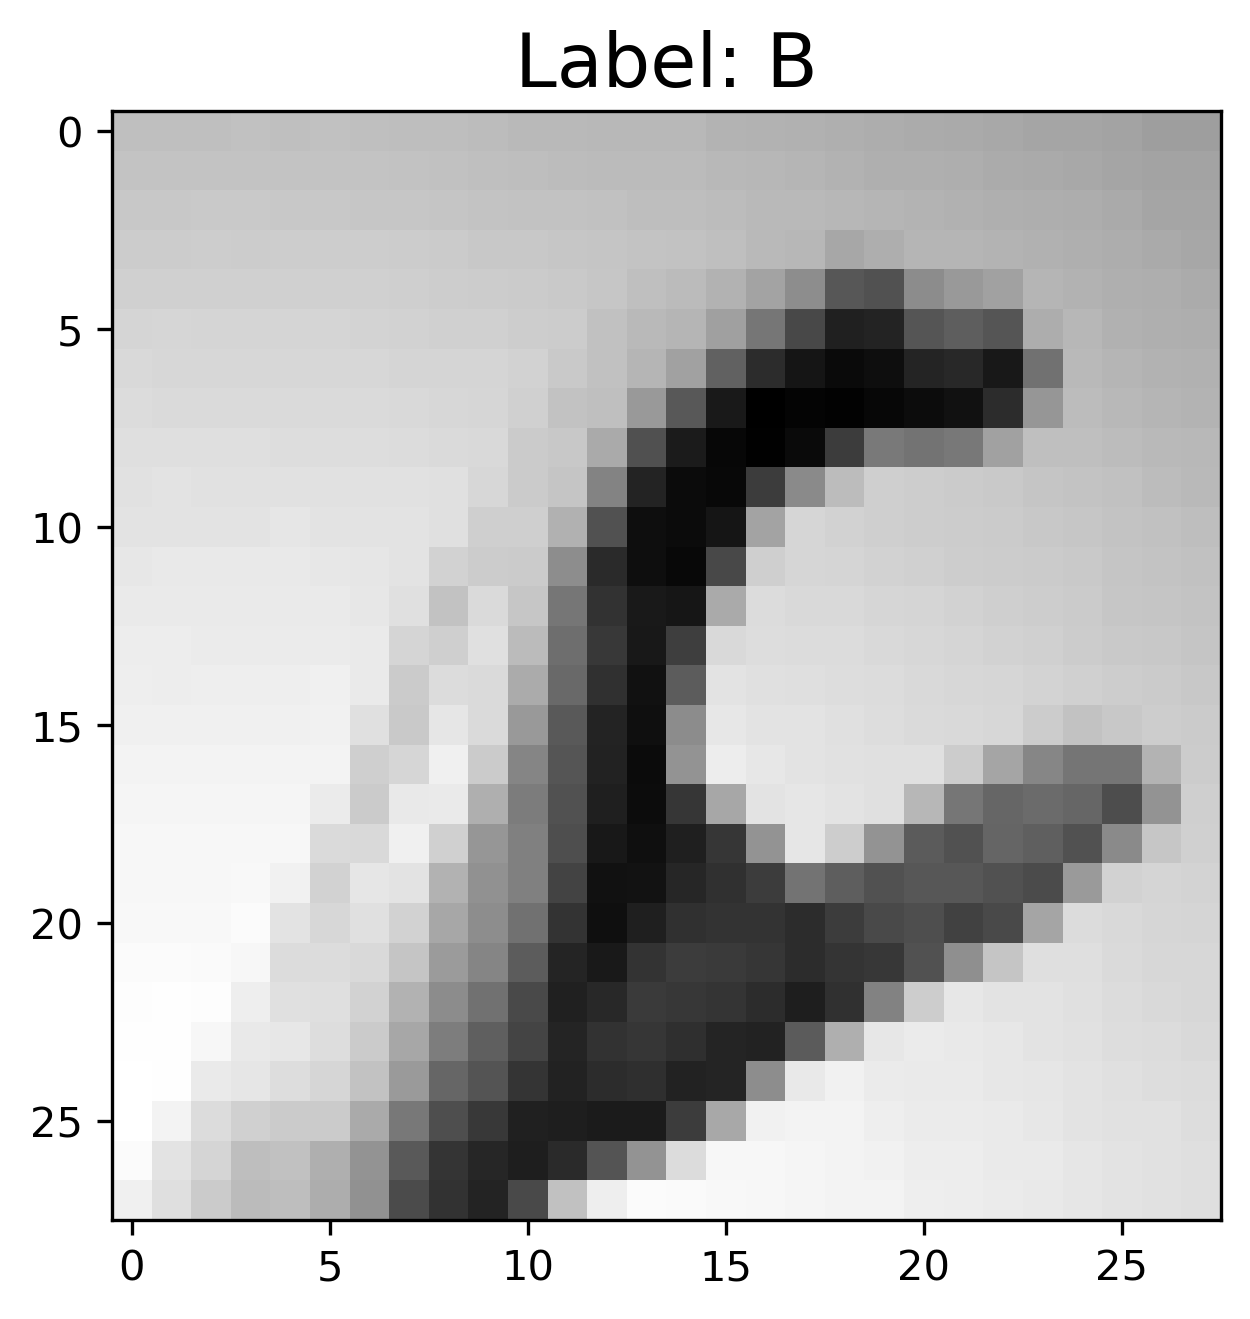
\includegraphics[height=0.31\linewidth]{../HW3_1/Sample6.png}}
		\subfigure[]{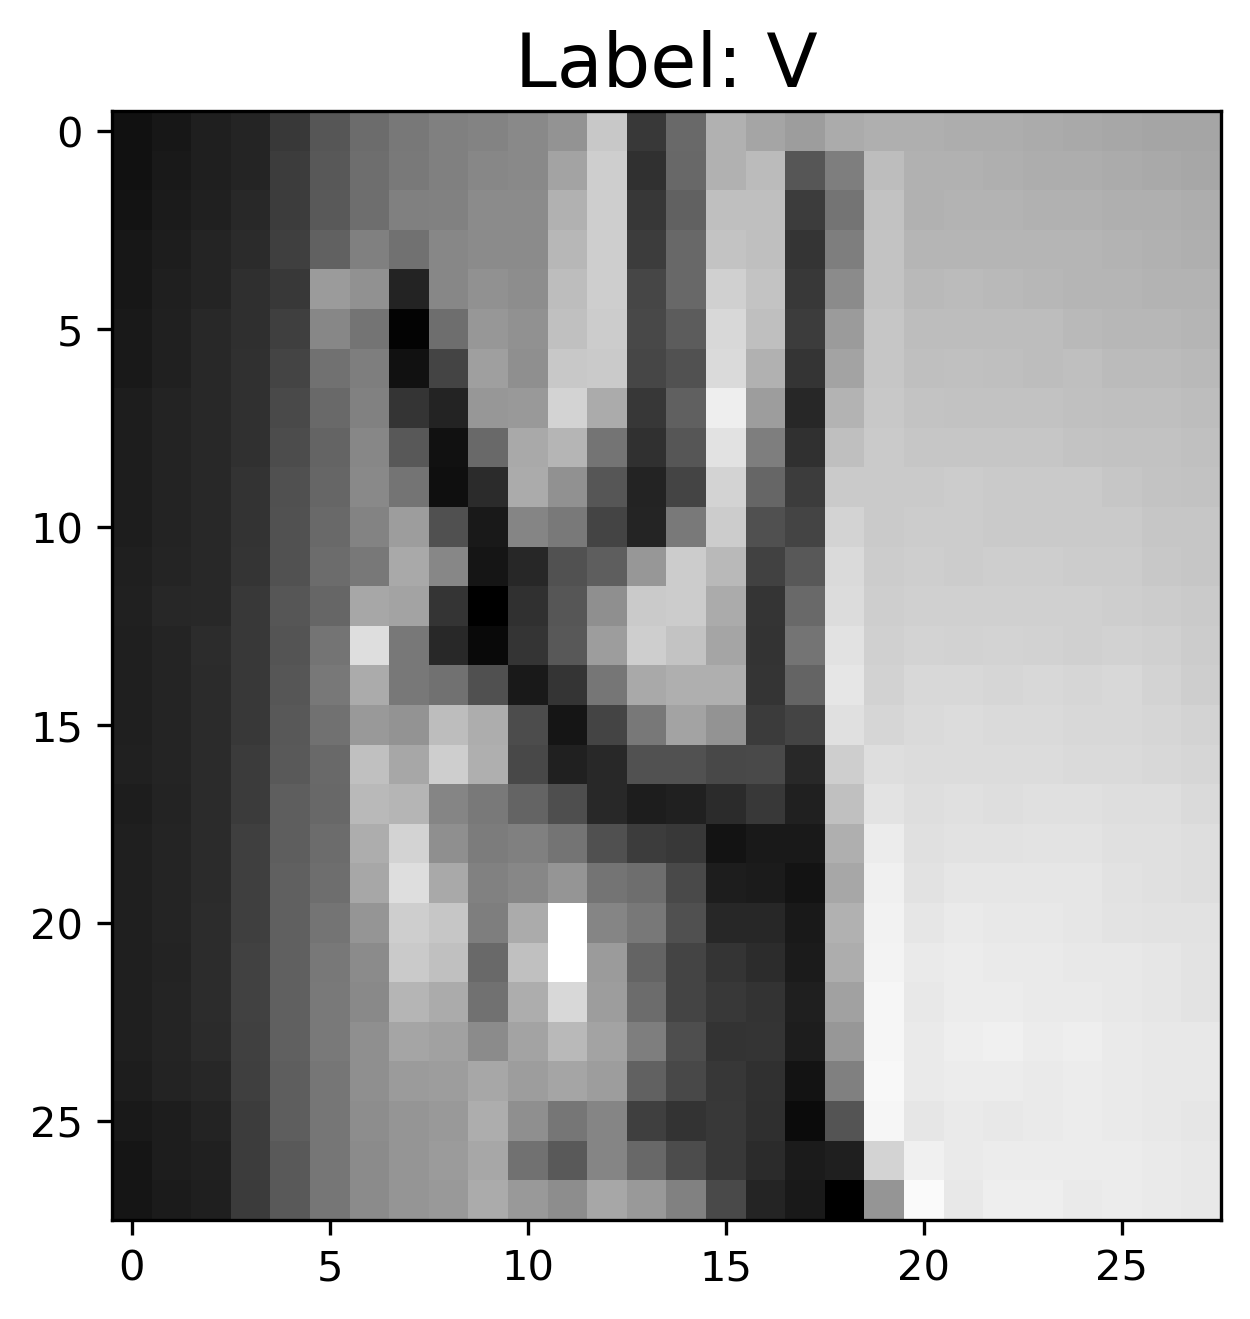
\includegraphics[height=0.31\linewidth]{../HW3_1/Sample7.png}}
		\caption{تصویر ۷ عدد از داده‌ها به صورت تصادفی}
		\label{fig:random_samples}
	\end{figure*}\\
	\clearpage
	شبکه‌ی مورد نظر با استفاده از دو بهینه‌ساز و دو نرخ یادگیری تمرین داده خواهد شد که نتایج در ادامه خواهد آمد.
	\begin{itemize}
		\item \lr{SGD ($\eta = 0.9$)}\\
		نمودار خطا و دقت در 
		\autoref{fig:sgd1}
		نشان داده شده است.
		\begin{figure}[!h]
			\centerline{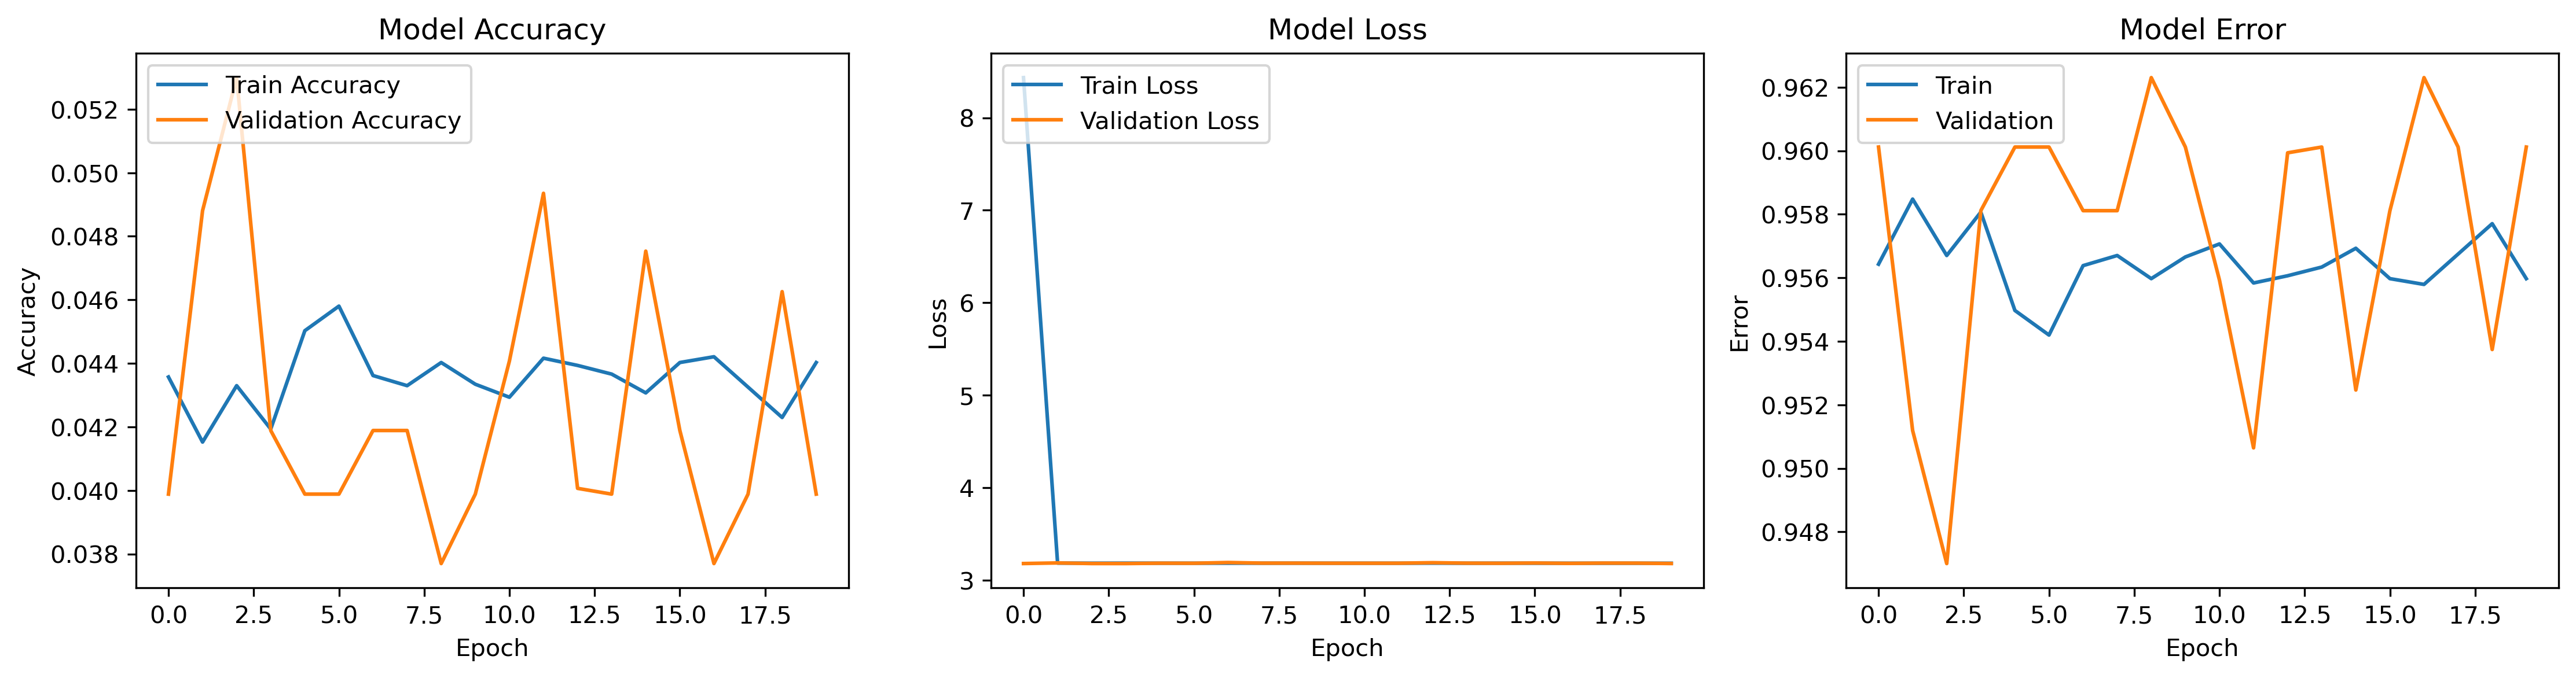
\includegraphics[width=1\linewidth]{../HW3_1/sgd1.png}}
			\caption{نمودار خطا، هزینه و دقت - بهینه‌ساز \lr{SGD} با $\eta=0.9$}
			\label{fig:sgd1}
		\end{figure}\\
		از جایی که نرخ یادگیری بالا است، دیده می‌شود که مدل به دقت خوبی نمیرسد. چنانچه این نرخ پایین بیاید می‌توان مدل را بهتر آموزش داد. ماتریس آشفتگی در
		\autoref{fig:sgd1_cm}
	آمده است.
		\begin{figure}[!h]
			\centerline{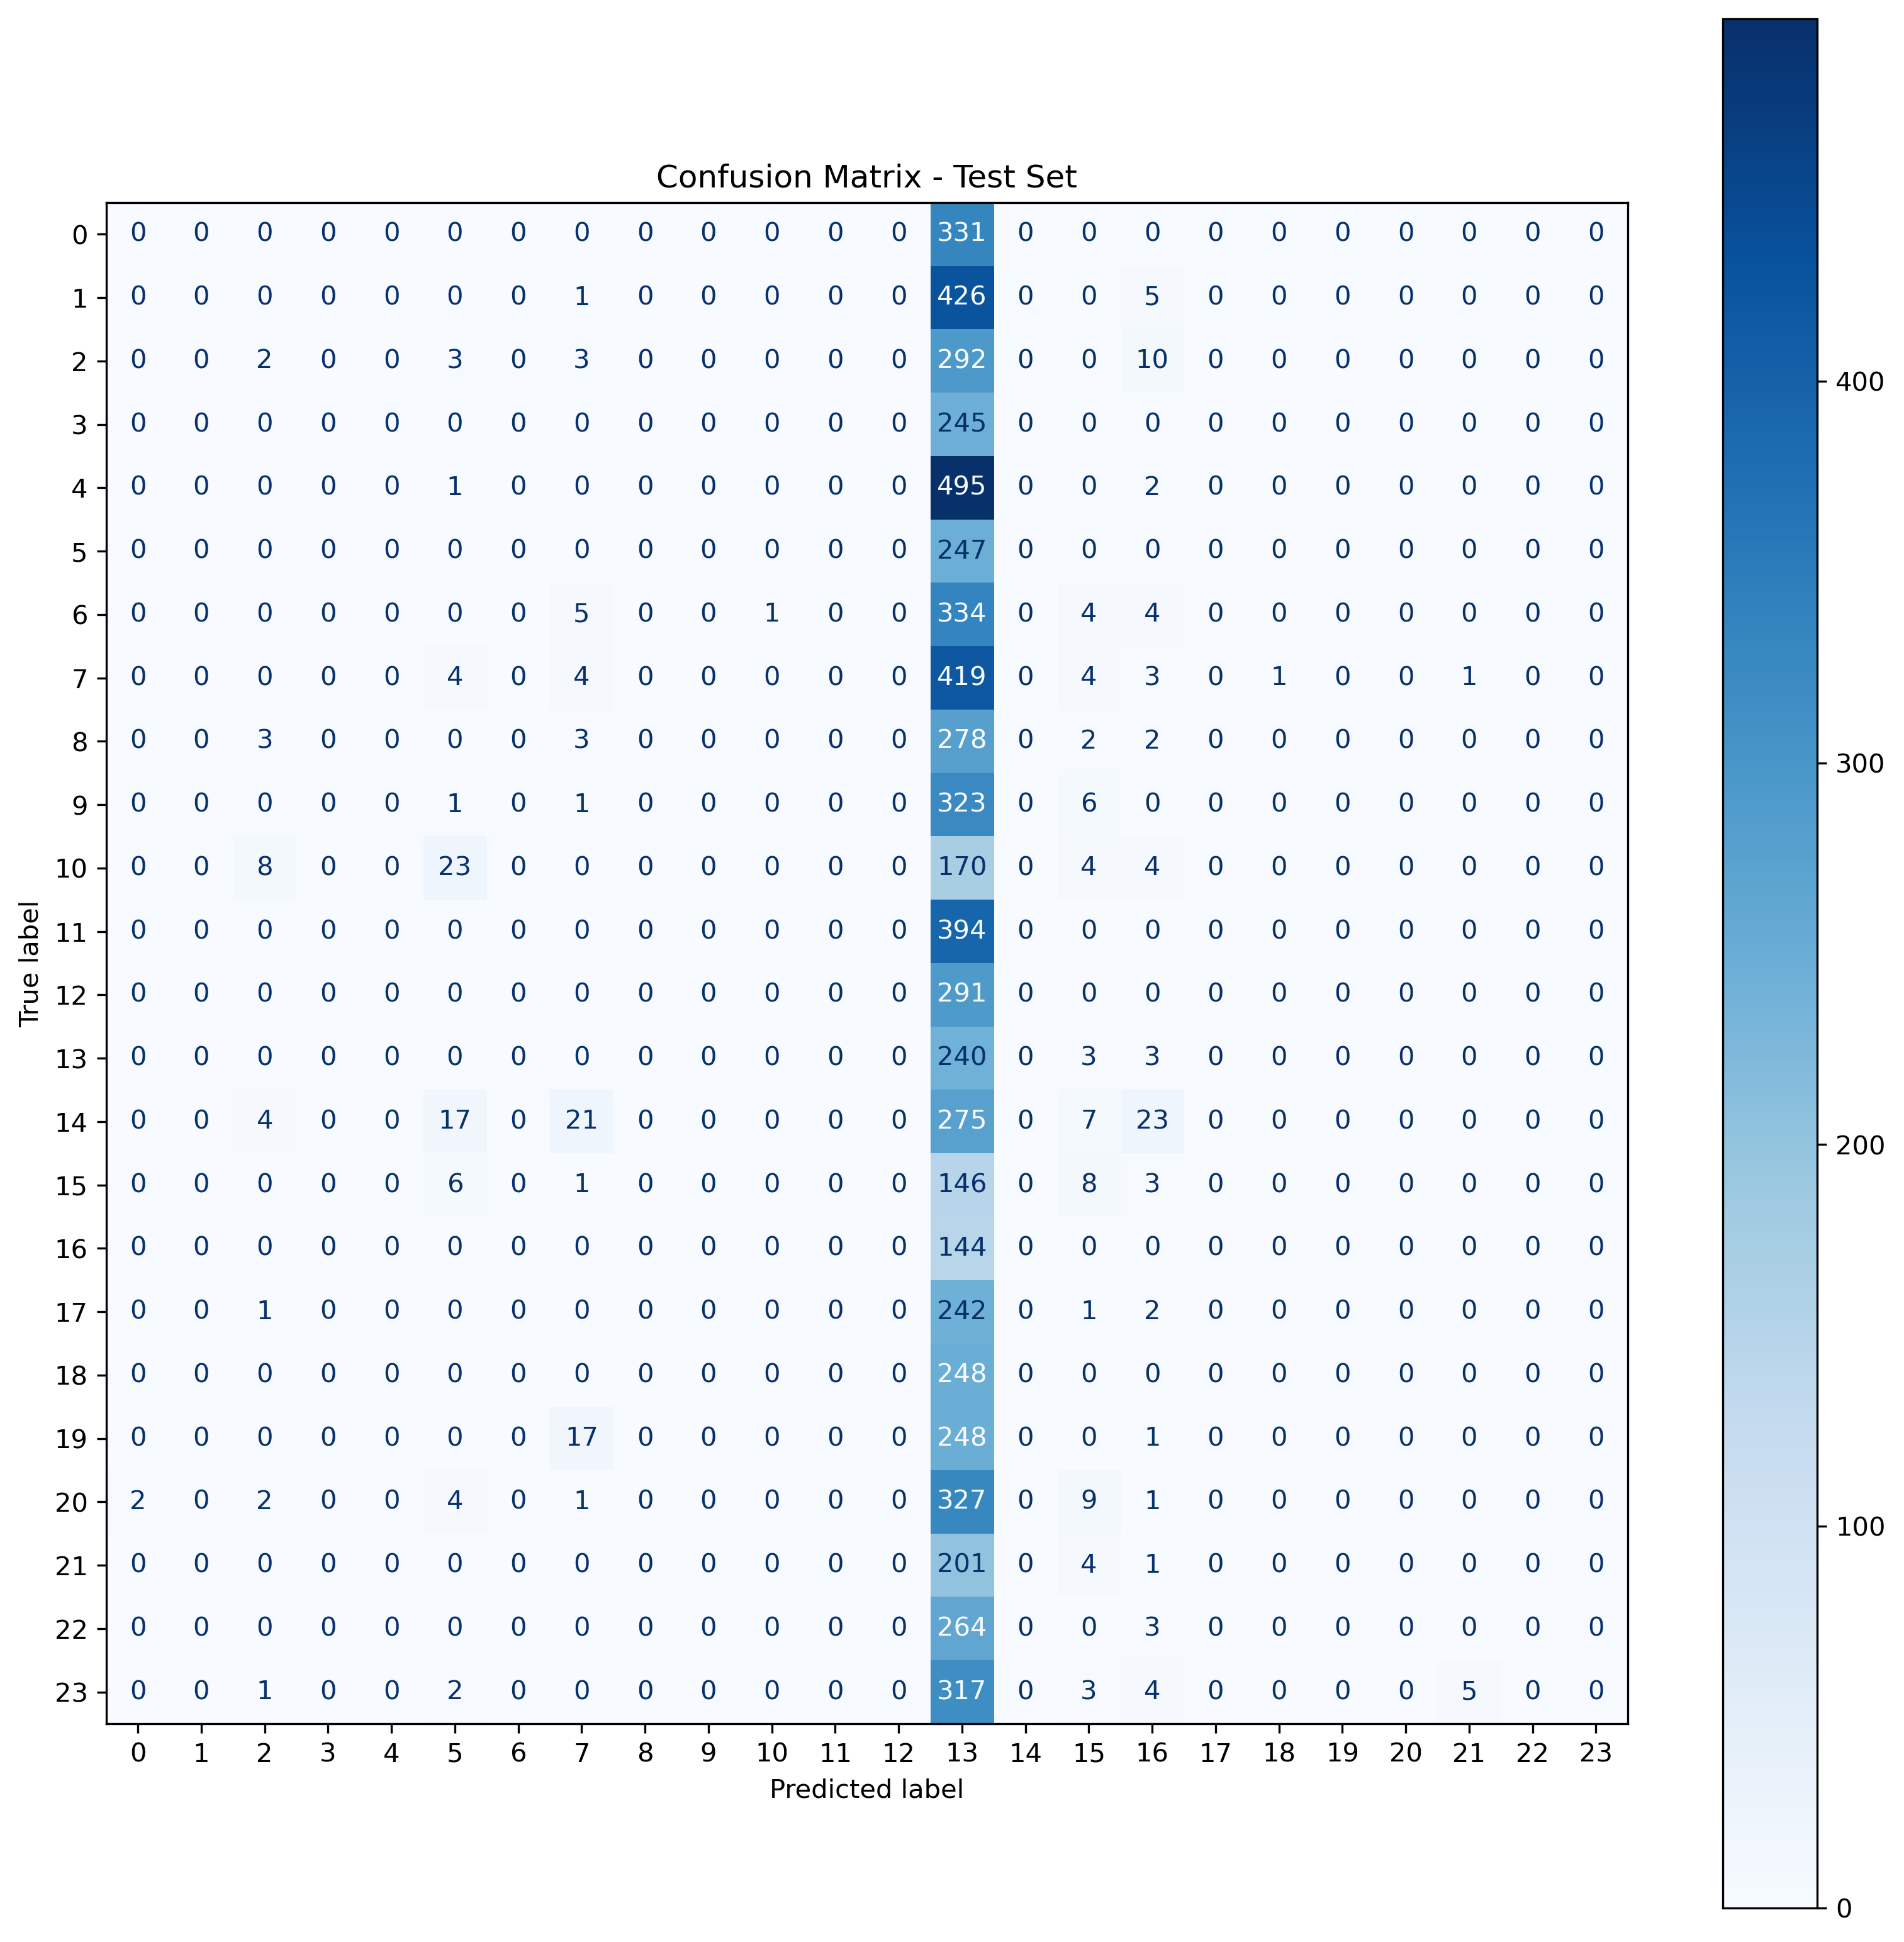
\includegraphics[width=0.5\linewidth]{../HW3_1/sgd1 cm.png}}
			\caption{ماتریس آشفتگی - بهینه‌ساز \lr{SGD} با $\eta=0.9$}
			\label{fig:sgd1_cm}
		\end{figure}\\
		\pagebreak
			\item \lr{SGD ($\eta = 0.01$)}\\
	نمودار خطا و دقت در 
	\autoref{fig:sgd2}
	نشان داده شده است.
	\begin{figure}[!h]
		\centerline{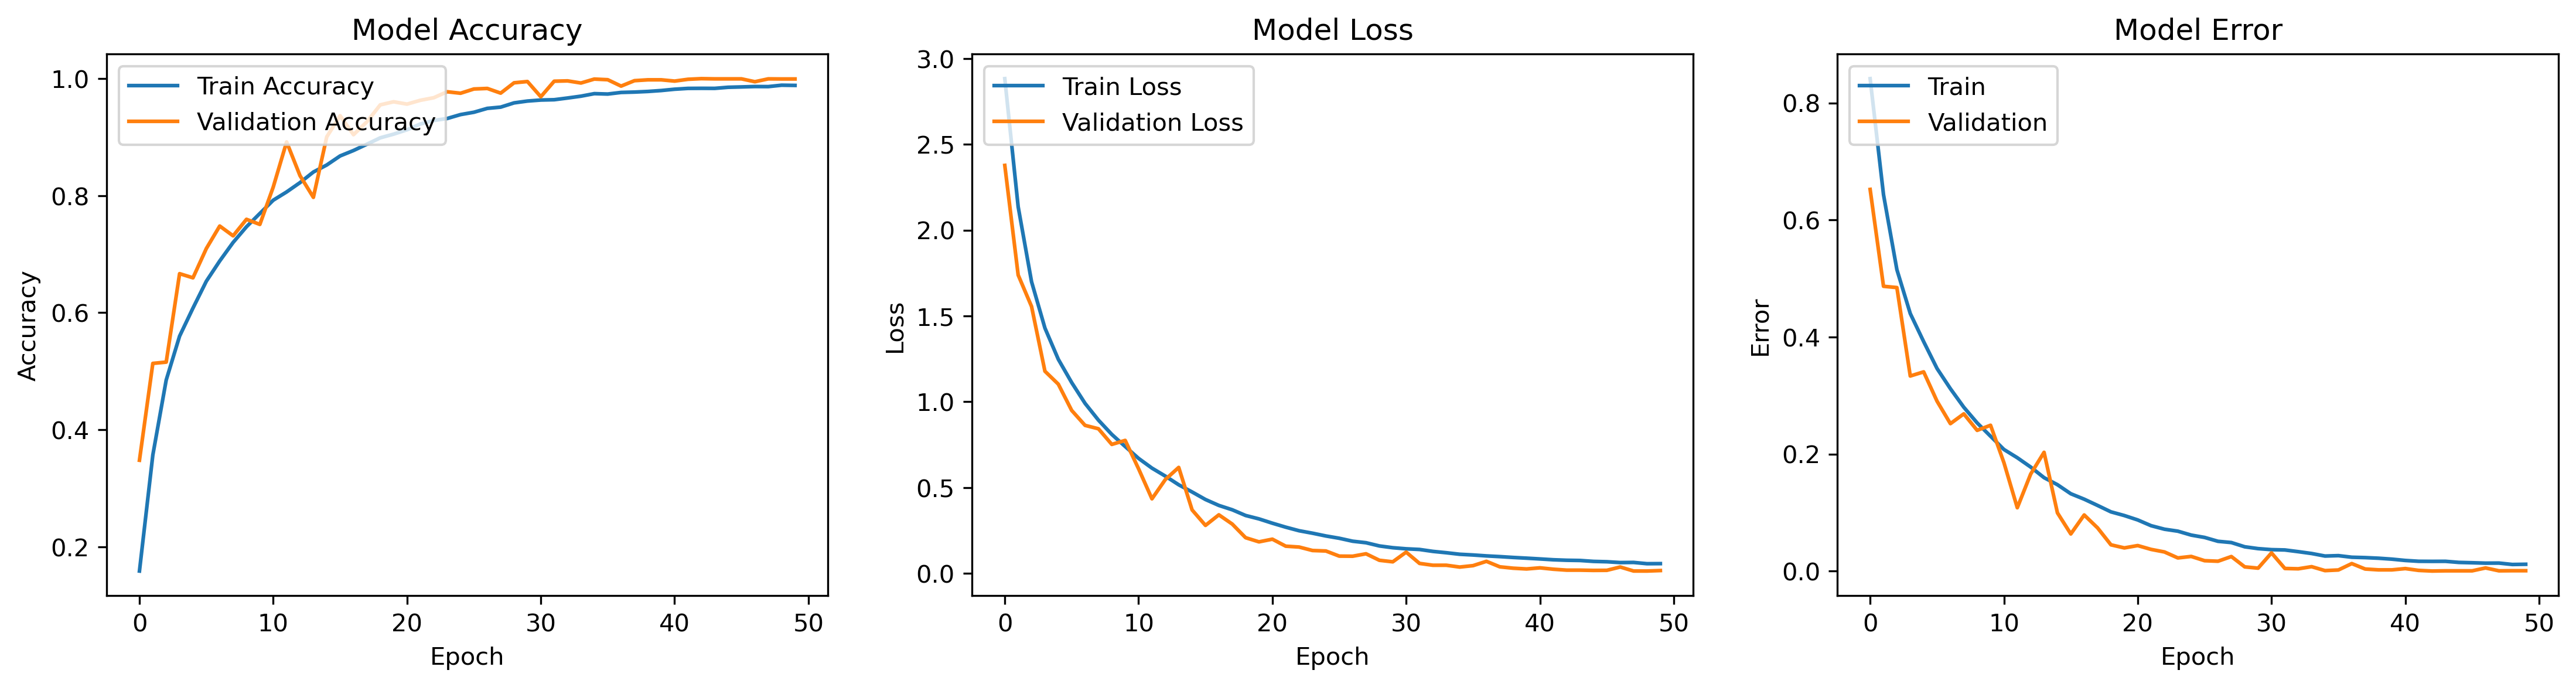
\includegraphics[width=1\linewidth]{../HW3_1/sgd2.png}}
		\caption{نمودار خطا، هزینه و دقت - بهینه‌ساز \lr{SGD} با $\eta=0.01$}
		\label{fig:sgd2}
	\end{figure}\\
	با کم کردن نرخ یادگیری، دیده می‌شود که حالا مدل در آموزش به همگرایی مناسبی می‌رسد. ماتریس آشفتگی در
	\autoref{fig:sgd2_cm}
	آمده است.
	\begin{figure}[!h]
		\centerline{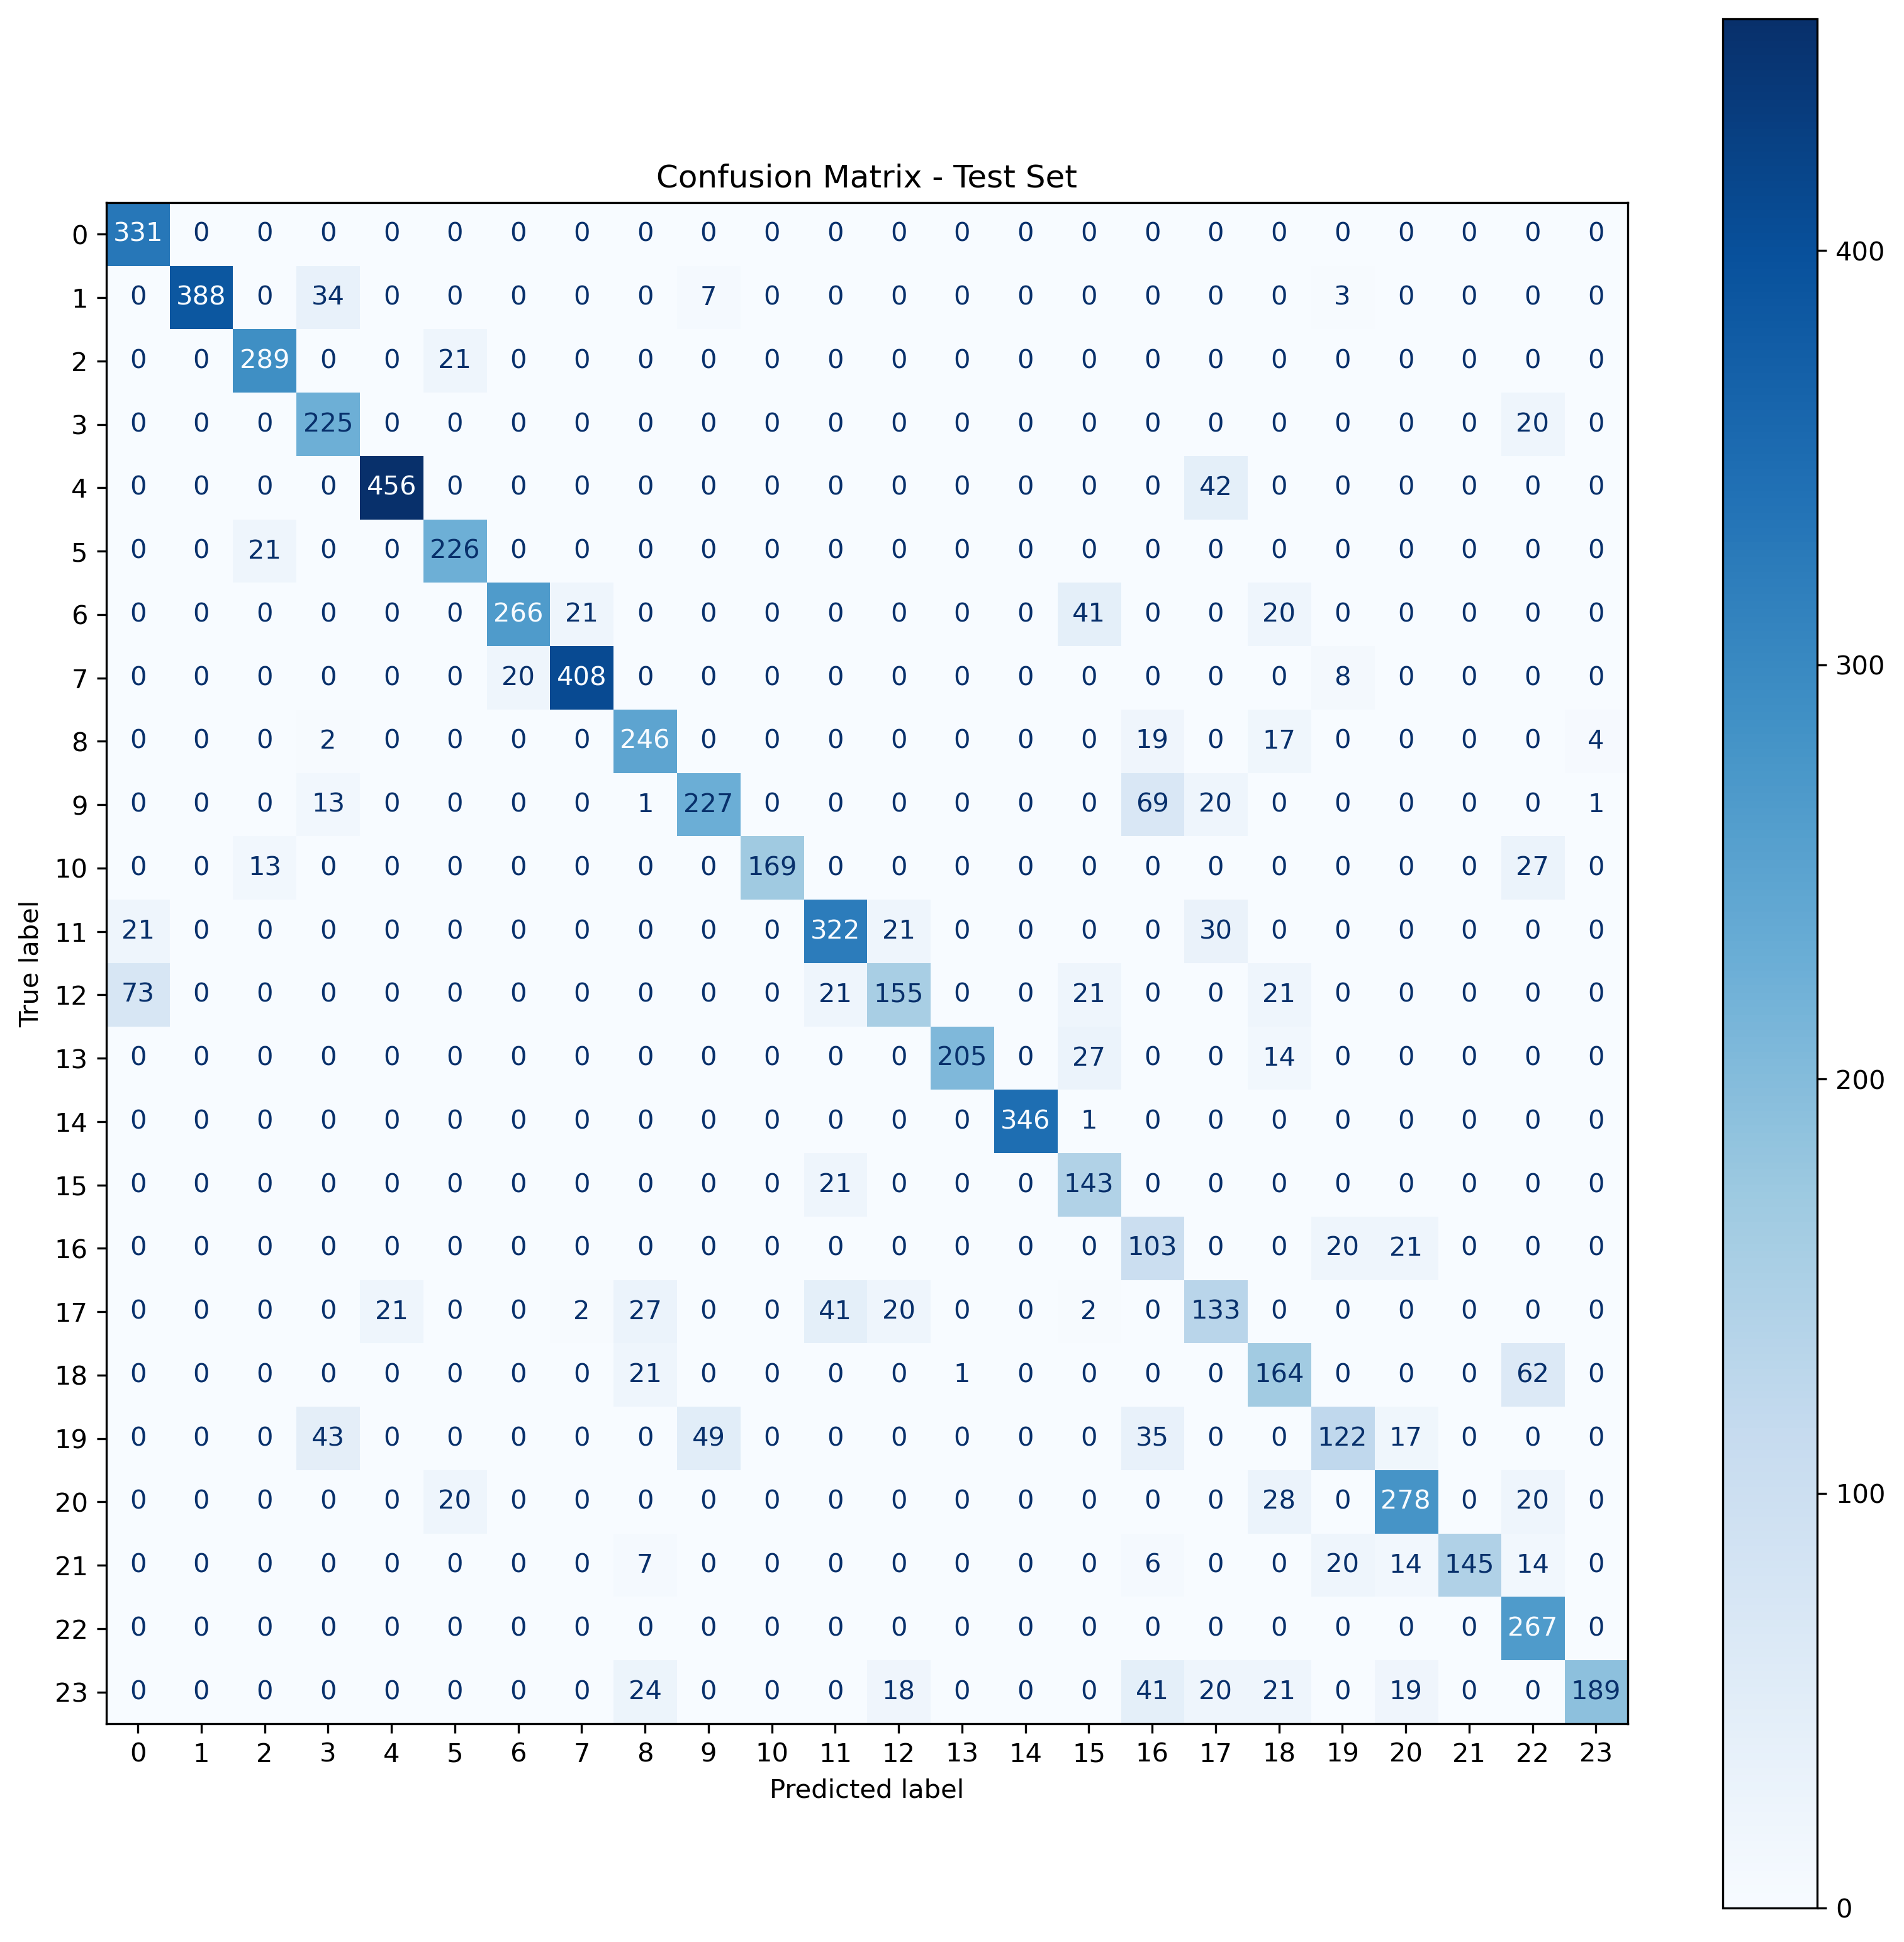
\includegraphics[width=0.5\linewidth]{../HW3_1/sgd2 cm.png}}
		\caption{ماتریس آشفتگی - بهینه‌ساز \lr{SGD} با $\eta=0.01$}
		\label{fig:sgd2_cm}
	\end{figure}\\
	\pagebreak
			\item \lr{Adam ($\eta = 0.9$)}\\
	نمودار خطا و دقت در 
	\autoref{fig:adam1}
	نشان داده شده است.
	\begin{figure}[!h]
		\centerline{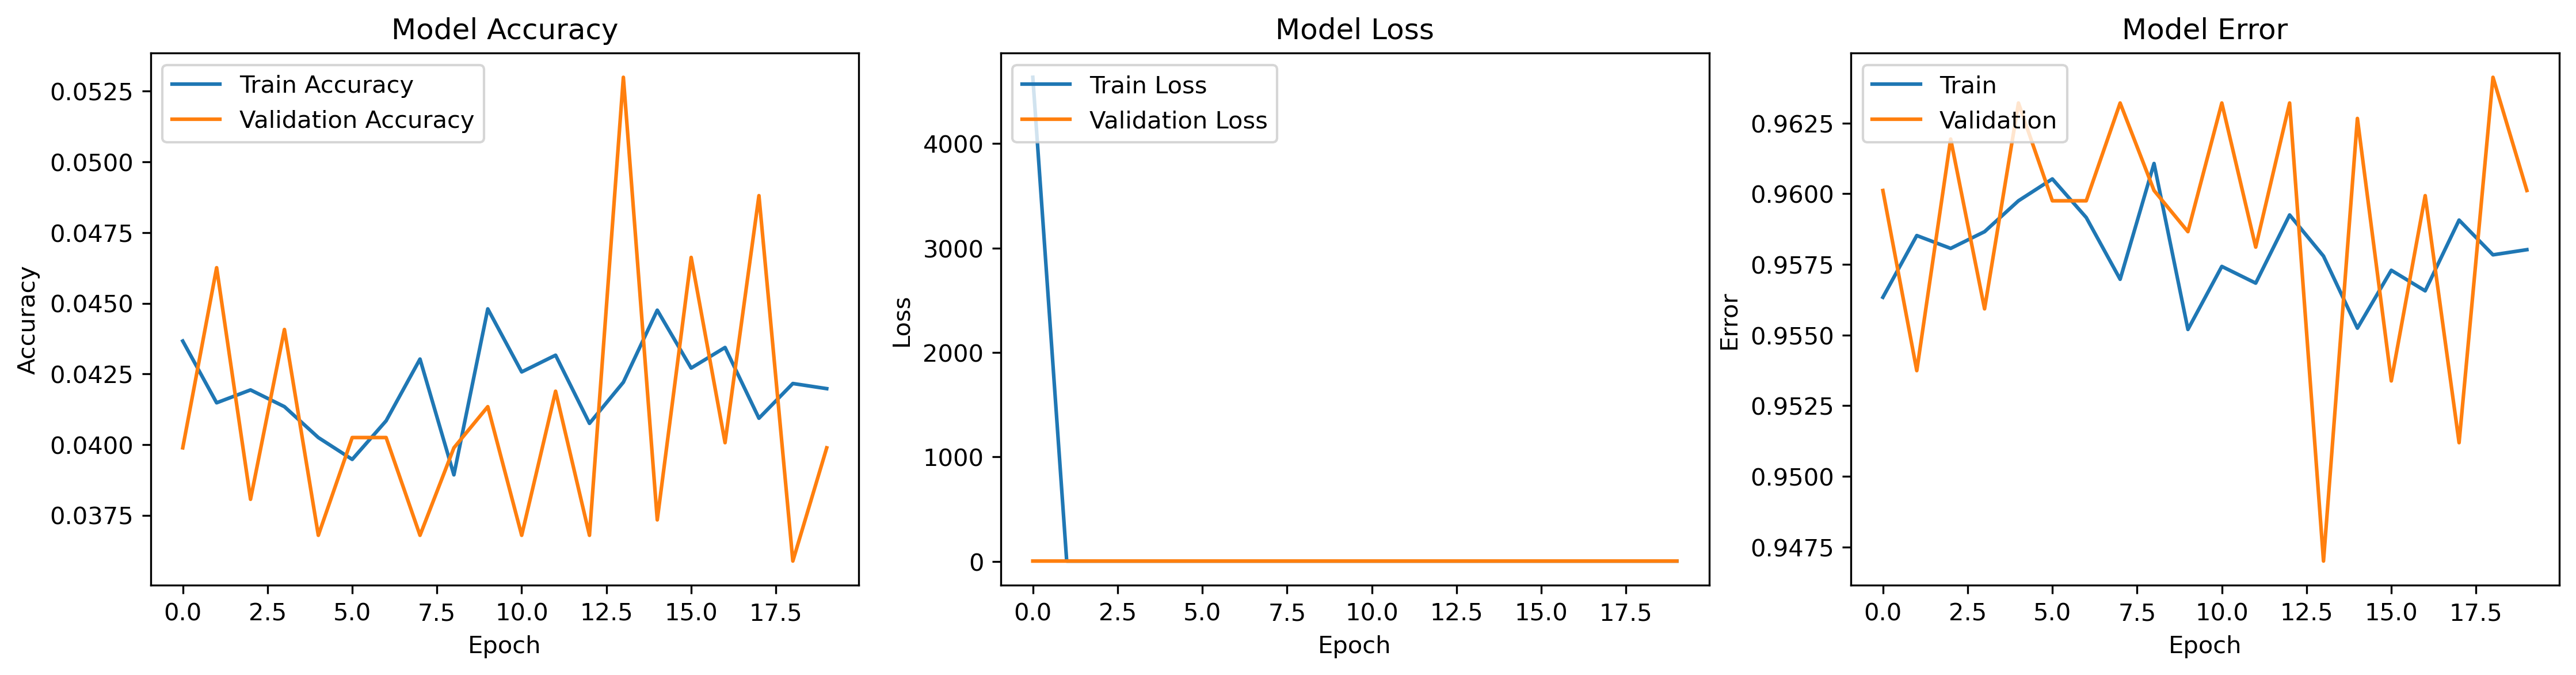
\includegraphics[width=1\linewidth]{../HW3_1/adam1.png}}
		\caption{نمودار خطا، هزینه و دقت - بهینه‌ساز \lr{Adam} با $\eta=0.9$}
		\label{fig:adam1}
	\end{figure}\\
	همانند حالت اول در بهینه‌ساز قبلی، این مدل نیز با نرخ یادگیری بالا همگرا نمی‌شود. ماتریس آشفتگی در
	\autoref{fig:adam1_cm}
	آمده است.
	\begin{figure}[!h]
		\centerline{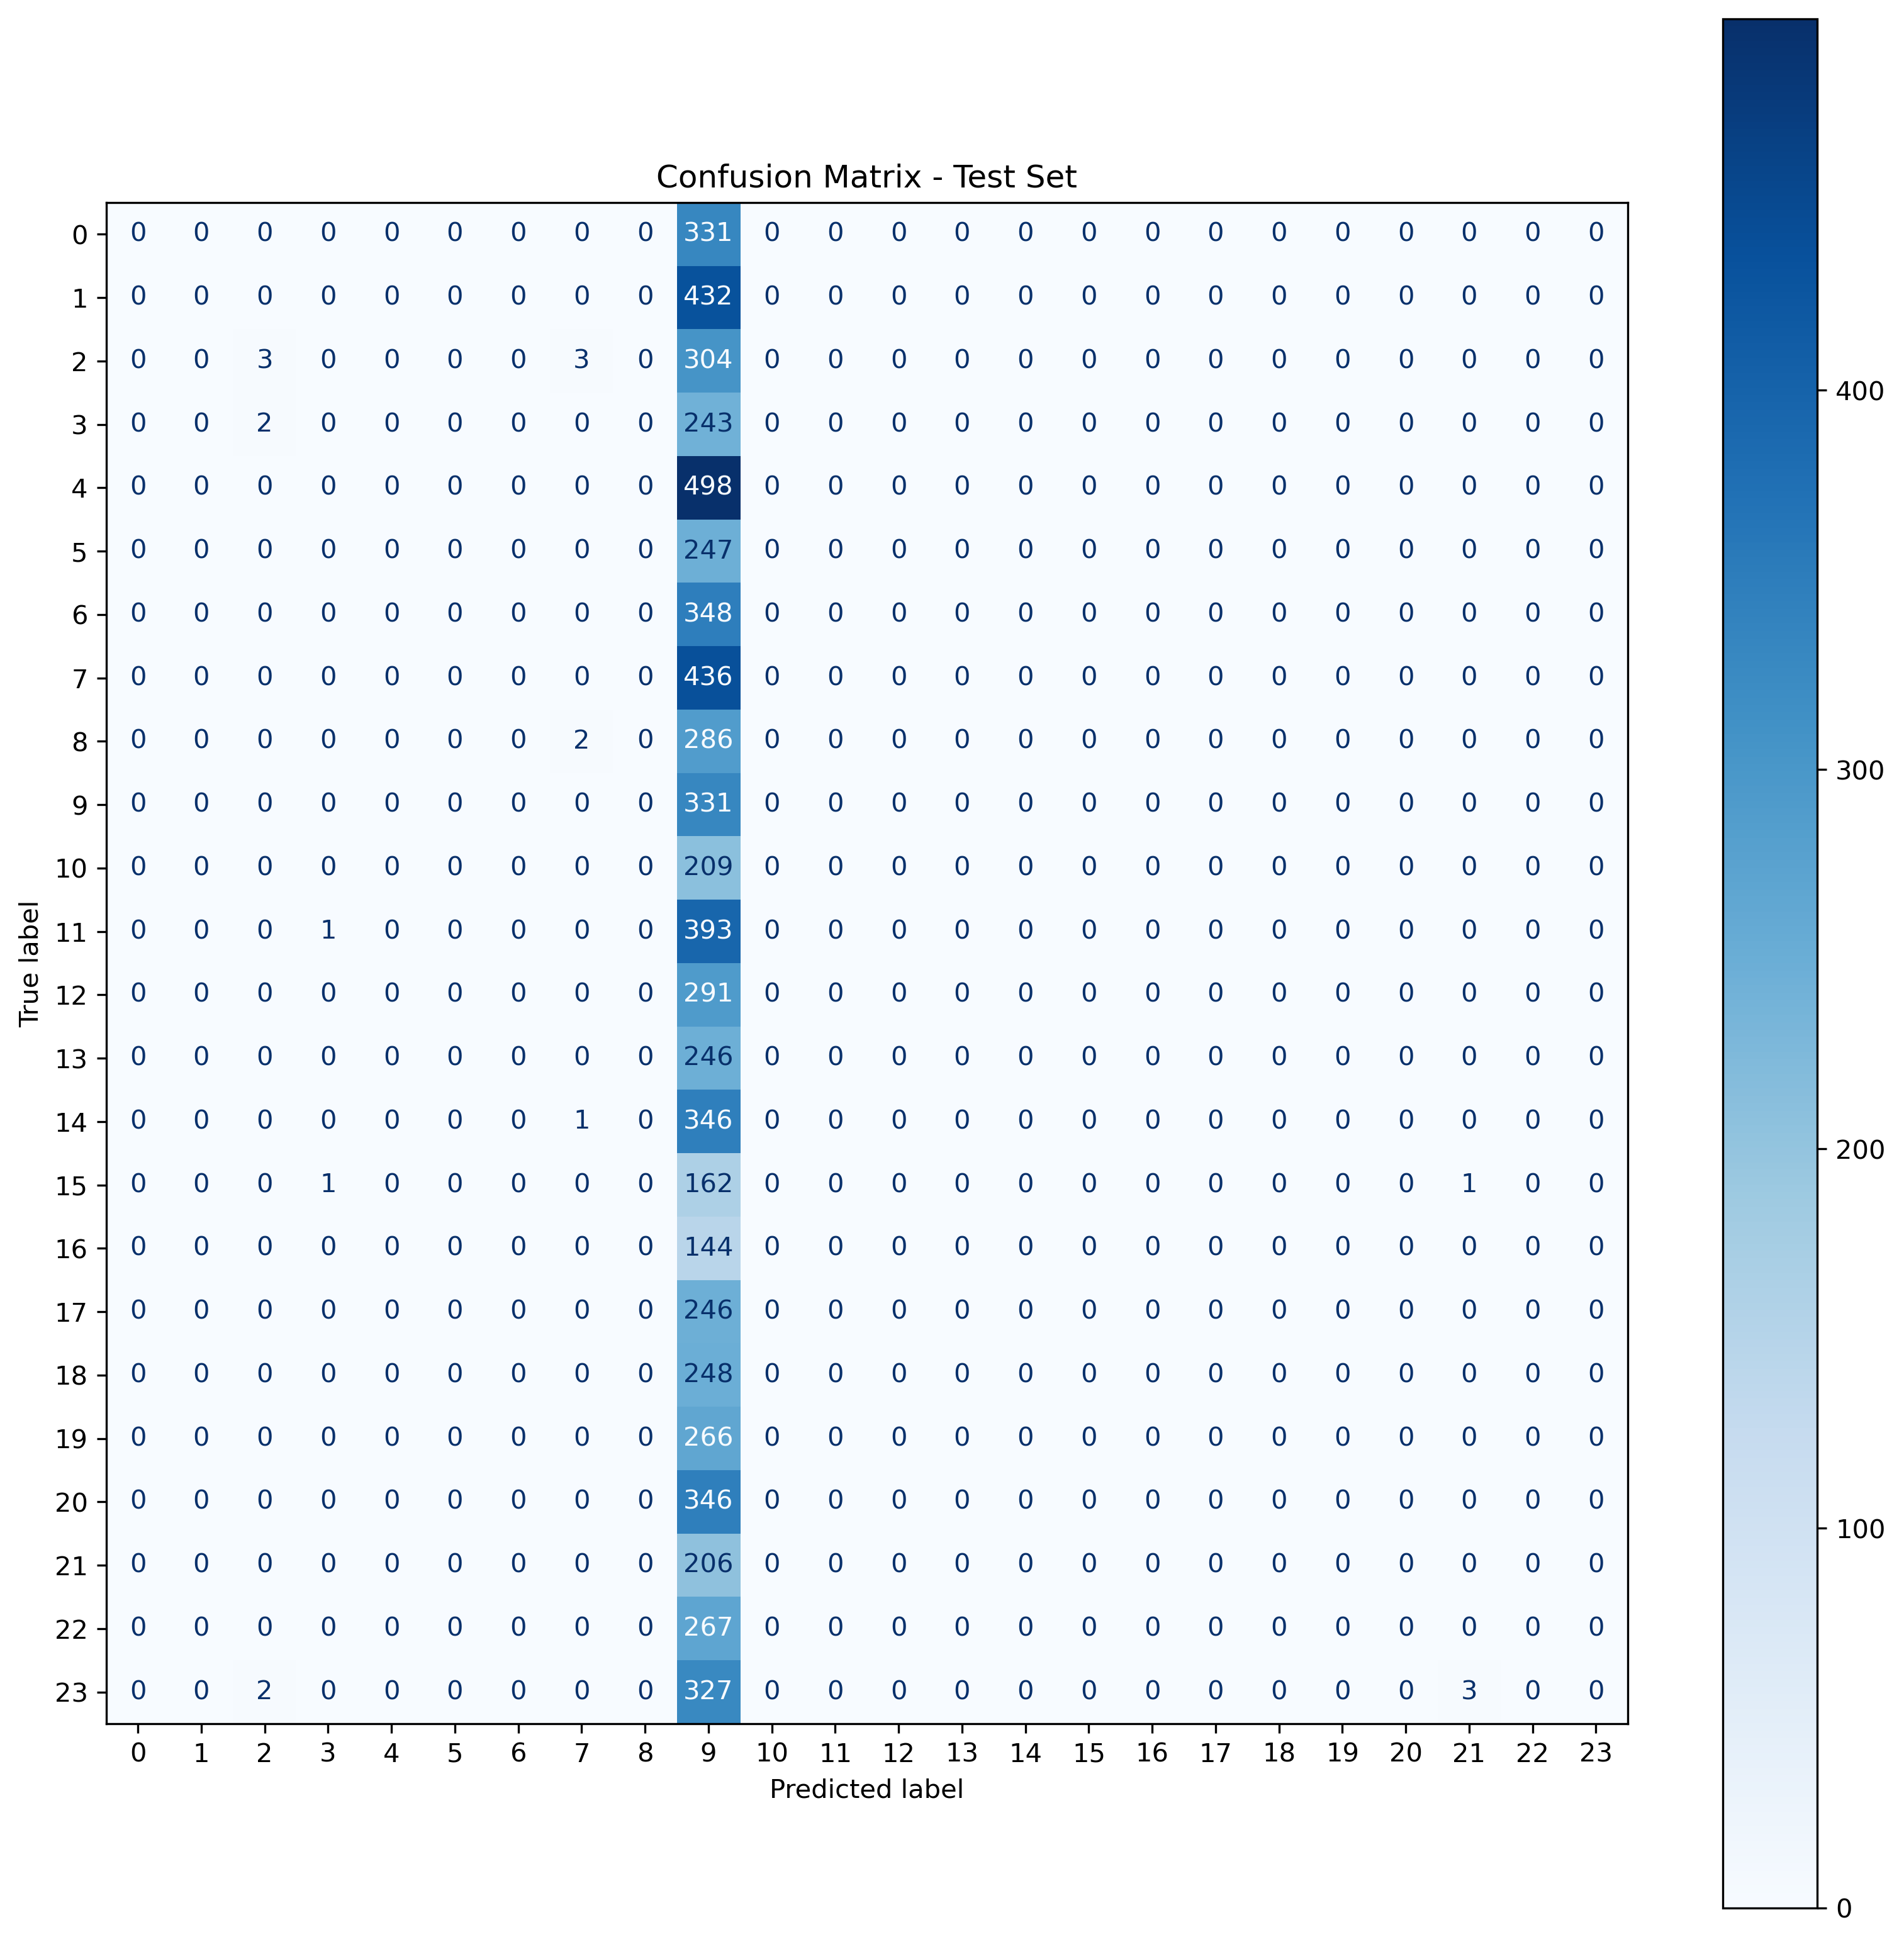
\includegraphics[width=0.5\linewidth]{../HW3_1/adam1 cm.png}}
		\caption{ماتریس آشفتگی - بهینه‌ساز \lr{Adam} با $\eta=0.9$}
		\label{fig:adam1_cm}
	\end{figure}\\
	\pagebreak
			\item \lr{Adam ($\eta = 0.01$)}\\
	نمودار خطا و دقت در 
	\autoref{fig:adam2}
	نشان داده شده است.
	\begin{figure}[!h]
		\centerline{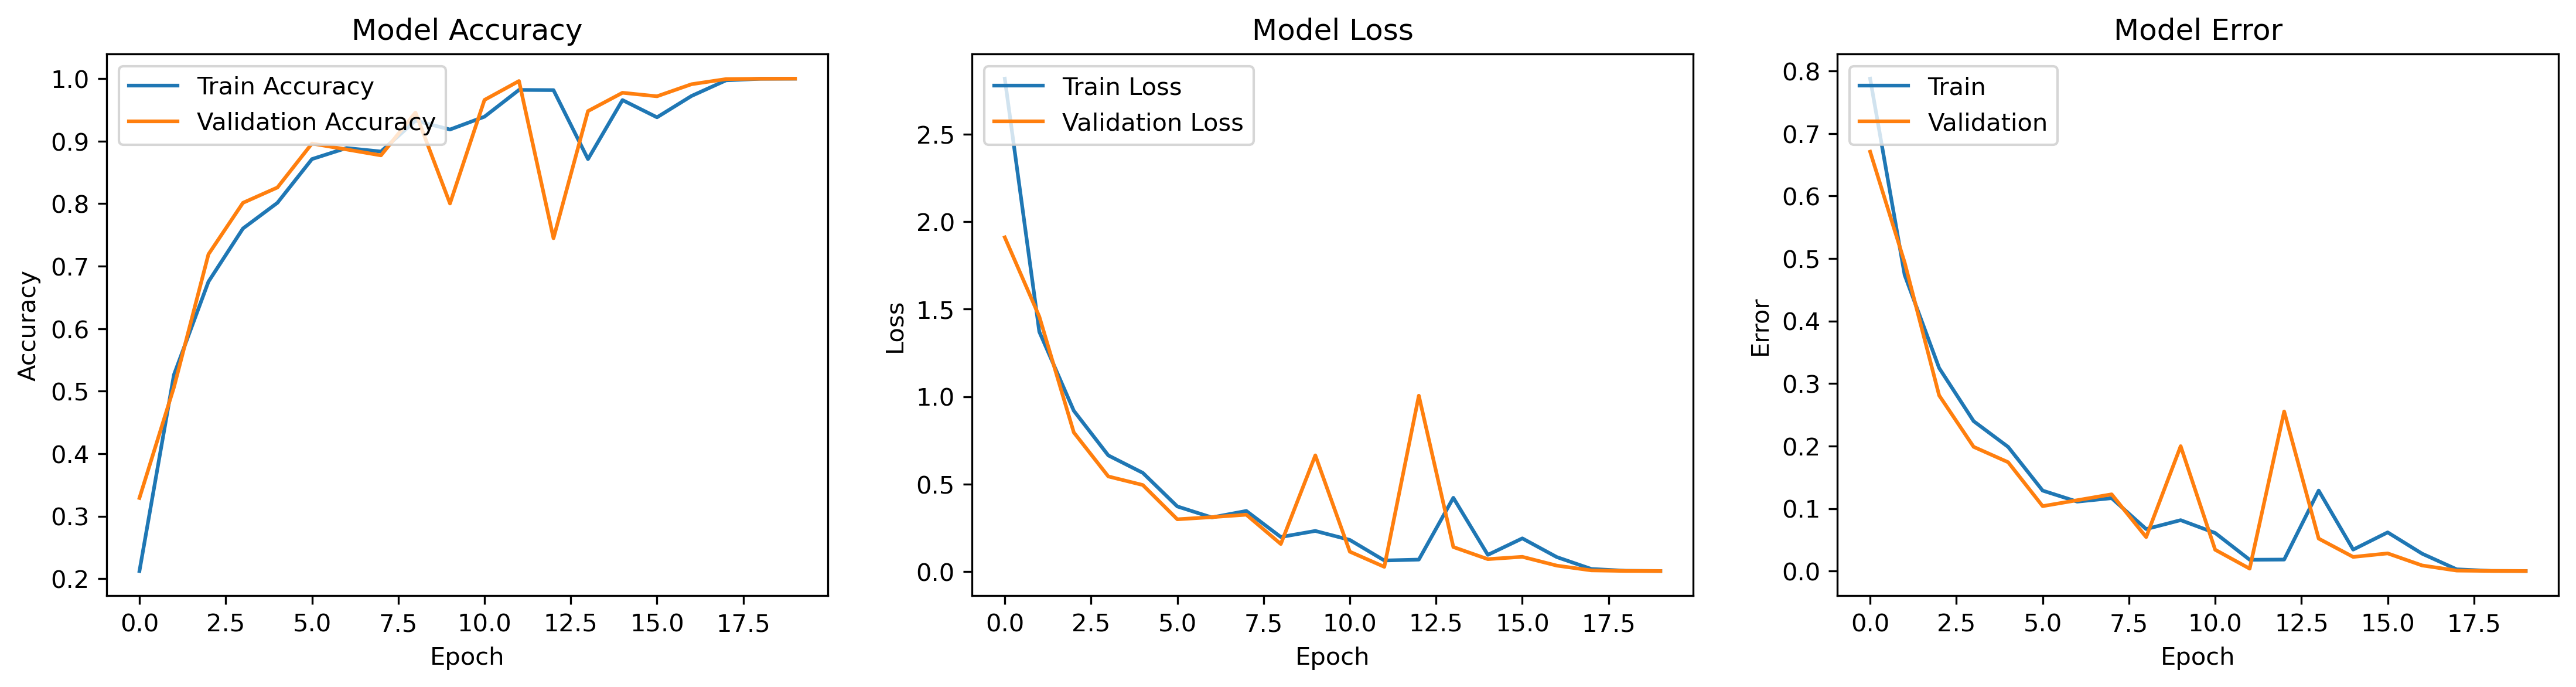
\includegraphics[width=1\linewidth]{../HW3_1/adam2.png}}
		\caption{نمودار خطا، هزینه و دقت - بهینه‌ساز \lr{Adam} با $\eta=0.01$}
		\label{fig:adam2}
	\end{figure}\\
	از جایی که نرخ یادگیری بالا است، دیده می‌شود که مدل به دقت خوبی نمیرسد. چنانچه این نرخ پایین بیاید می‌توان مدل را بهتر آموزش داد. ماتریس آشفتگی در
	\autoref{fig:adam1_cn}
	آمده است.
	\begin{figure}[!h]
		\centerline{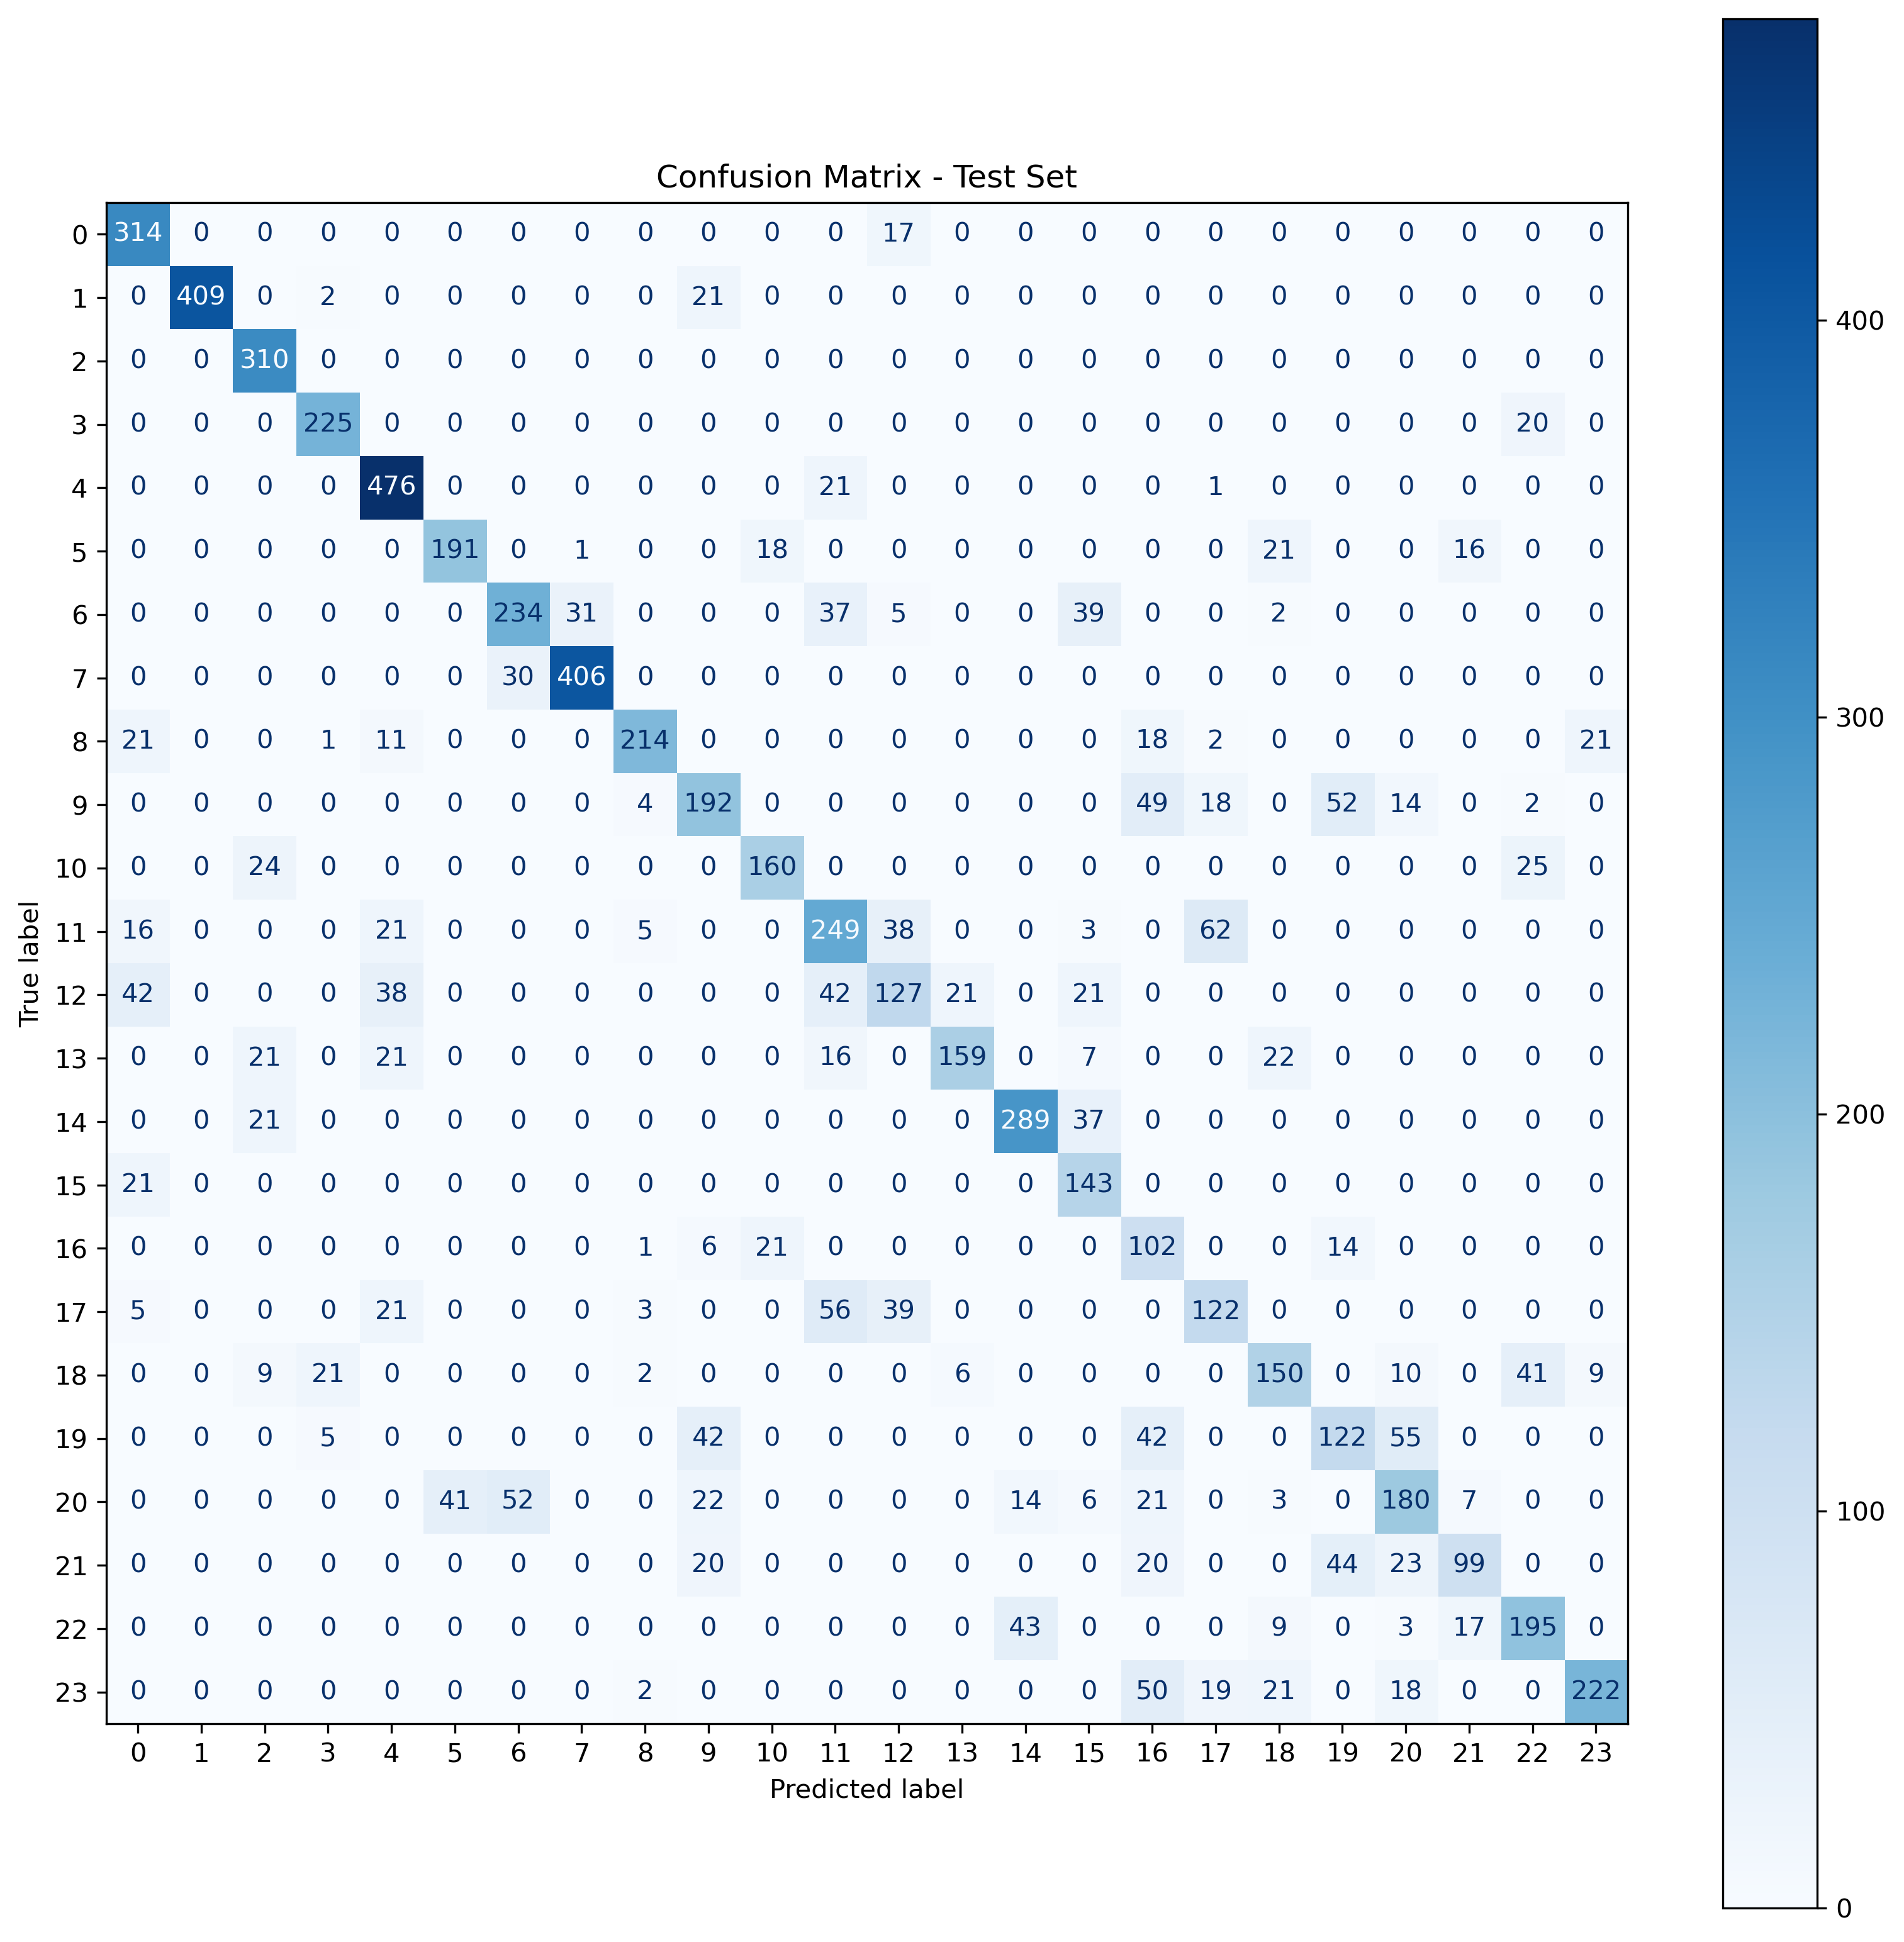
\includegraphics[width=0.5\linewidth]{../HW3_1/adam2 cm.png}}
		\caption{ماتریس آشفتگی - بهینه‌ساز \lr{Adam} با $\eta=0.9$}
		\label{fig:sgdcm}
	\end{figure}\\
	\pagebreak
	\end{itemize}
	در نهایت، دقت هر حالت در 
	\autoref{tab:accuracy1}
	به صورت تجمیعی آمده است.
	\begin{table}[h!]
		\caption{جمع‌بندی نتایج مدل‌ها برای پیش‌بینی دیابت}
		\begin{latin}
			\centering
			\begin{tabular}{|l|c|c|}
				\hline
				\textbf{Optimizer} & \textbf{Learning Rate} & \textbf{Test accuracy} \\ \hline
				SGD & 0.9 & 0.0365 \\ \hline
				SGD & 0.9 & 0.8044 \\ \hline
				Adam & 0.01 &  0.0465 \\ \hline
				Adam & 0.01 & 0.7279 \\ \hline
			\end{tabular}
		\end{latin}
		\label{tab:accuracy1} 
	\end{table}\\
	لازم به ذکر است که هنگام تمرین داده‌ها مشاهده شد که بهینه‌ساز \lr{Adam} با نرخ \lr{Dropout}  کمتر نسبت به \lr{SGD} بهتر همگرا می‌شود.
	\section{شبکه \lr{CNN}}
	به منظور دسته‌بندی تصاویر، استفاده از مدل‌ها \lr{CNN} در این قسمت بررسی می‌شود. ابتدا یک مدل با ساختار 
	\autoref{fig:CNN_structure}
	تشکیل داده می‌شود. این مدل از دو لایه پیچشی، لایه‌های انبایشی، \lr{Batch Normalization} و یک لایه پنهان \lr{Dense} تشکیل شده است. در خروجی از تابع فعال‌سازی \lr{Softmax} استفاده شده است که در نهایت مقدار یکی از کلاس‌ها را با عدد ۱ و سایر را با صفر برمی‌گرداند.
	\begin{figure}[!h]
		\centerline{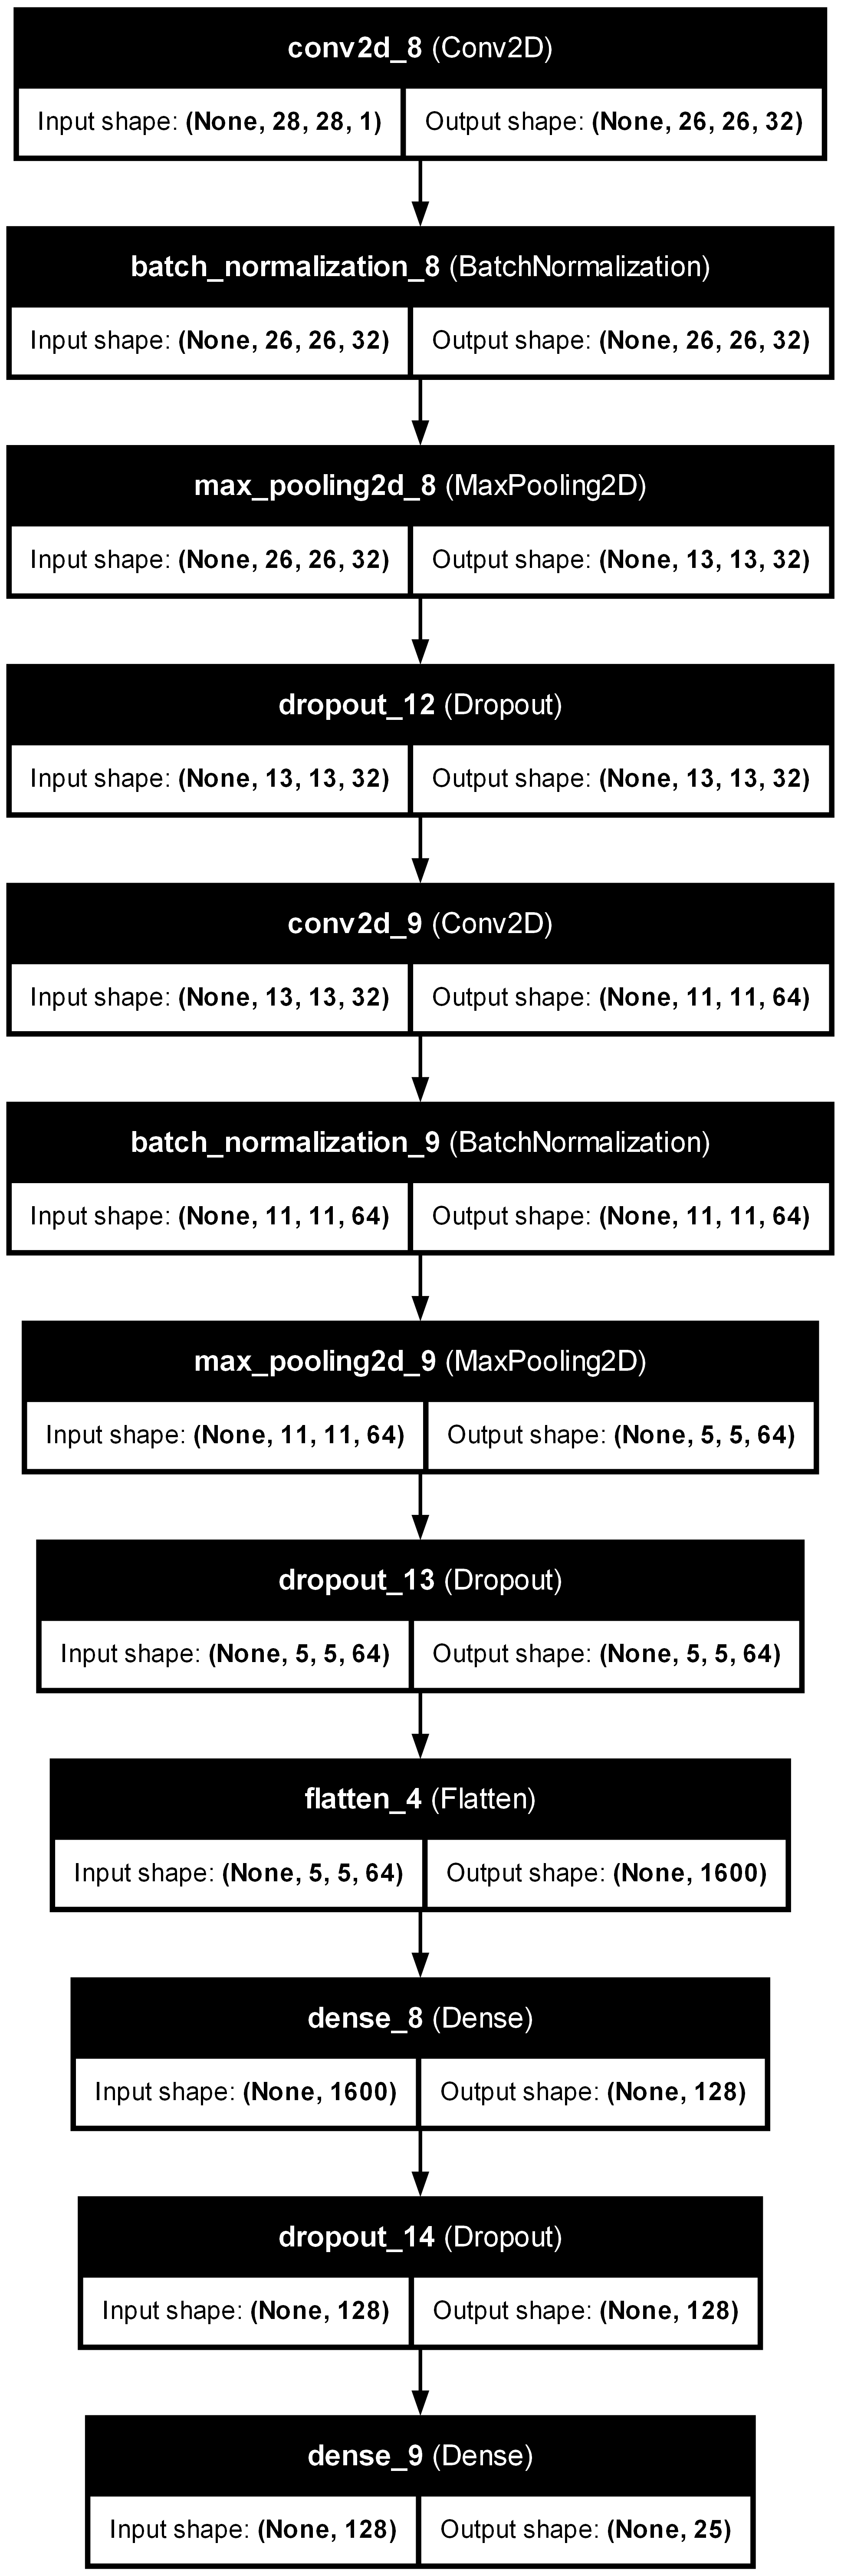
\includegraphics[width=0.3\linewidth]{../HW3_2/model_structure.png}}
		\caption{}
		\label{fig:CNN_structure}
	\end{figure}\\
	برای بهینه‌ساز مدل از الگوریتم \lr{Adam} استفاده می‌شود. دقت نهایی مدل برابر با $0.8599$ می‌باشد. نمودار‌های خطا و دقت در
	\autoref{fig:cnn1}
	و ماتریس آشفتگی در
	\autopageref{fig:cnn1_cm}
	آمده‌اند.
	\begin{figure}[!h]
		\centerline{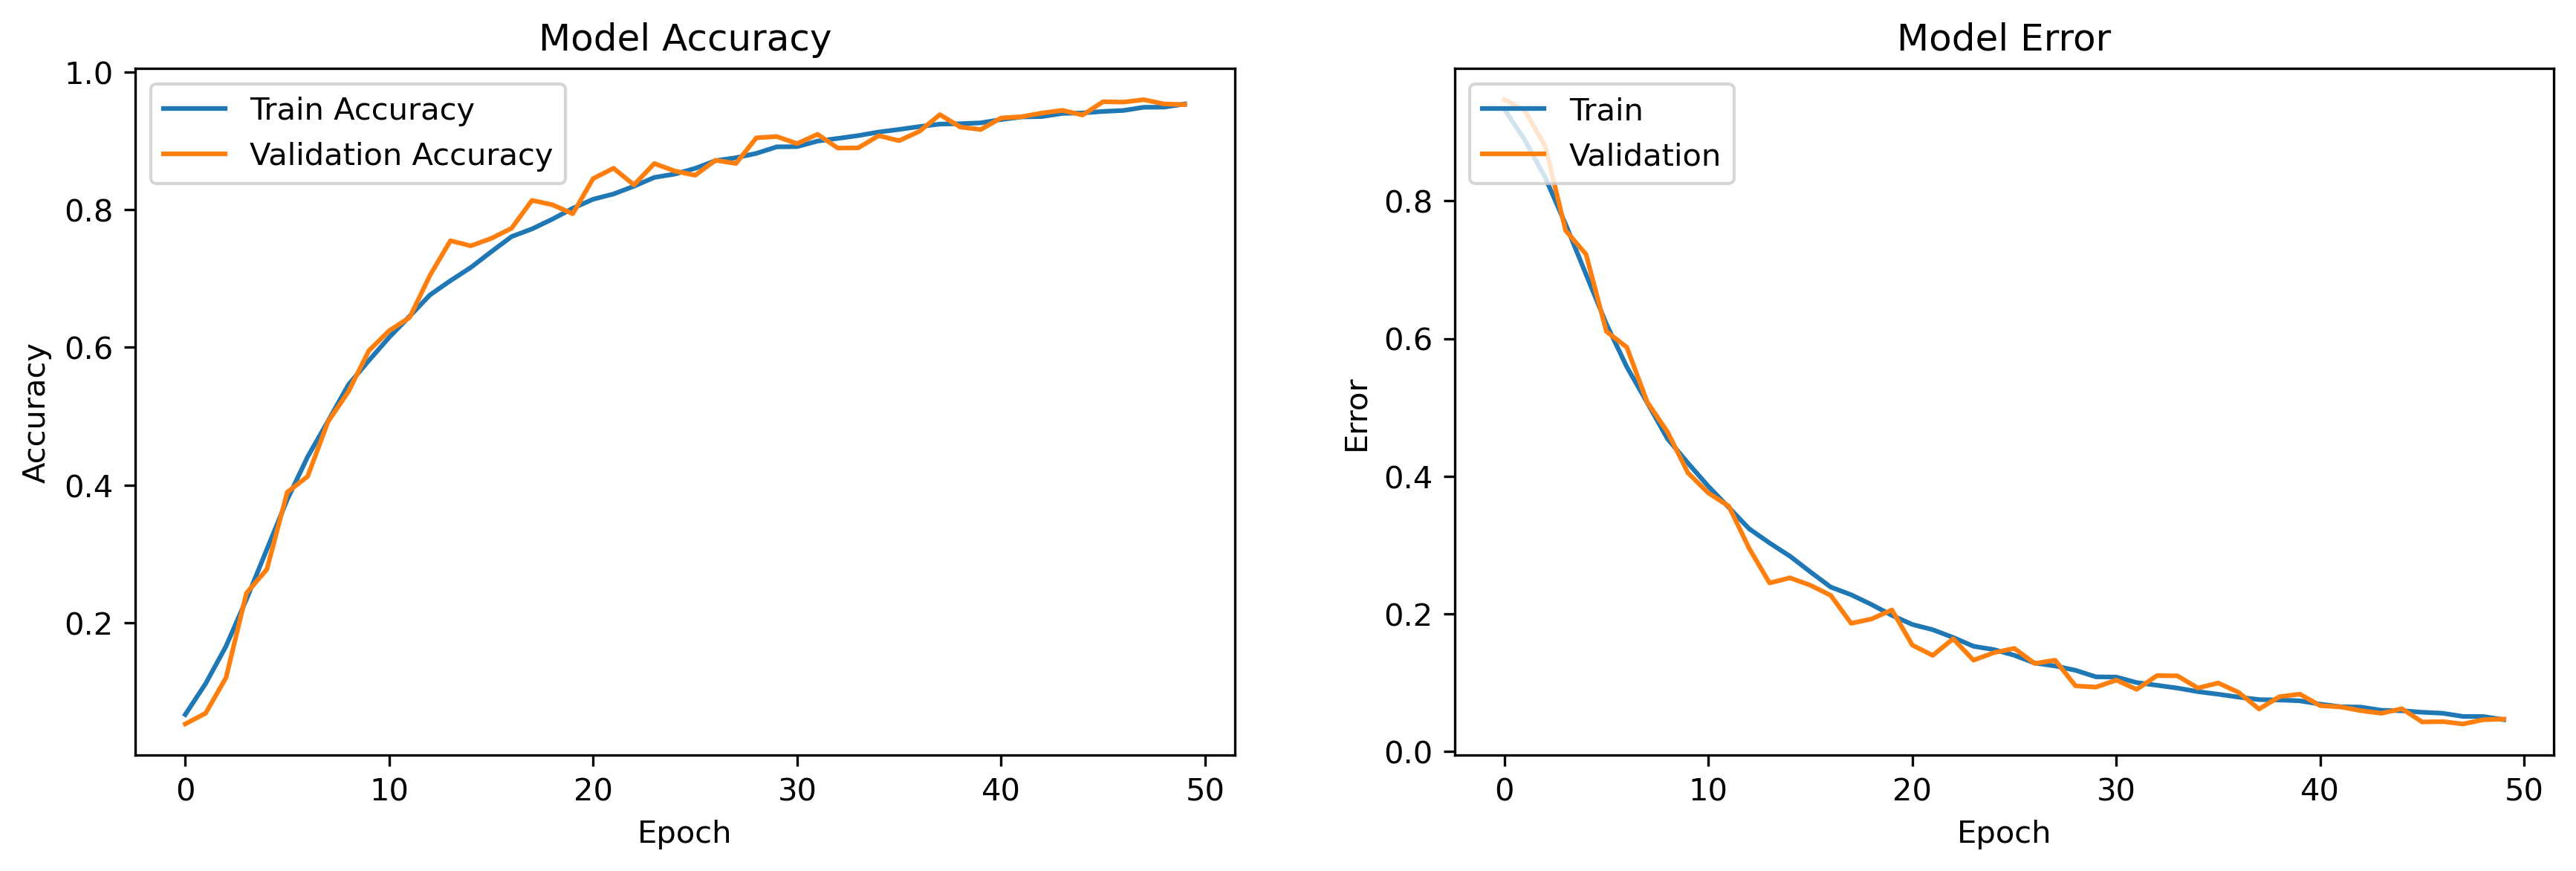
\includegraphics[width=1\linewidth]{../HW3_2/cnn1.png}}
		\caption{نمودار خطا و دقت  - مدل \lr{CNN}}
		\label{fig:cnn1}
	\end{figure}
	\begin{figure}[!h]
		\centerline{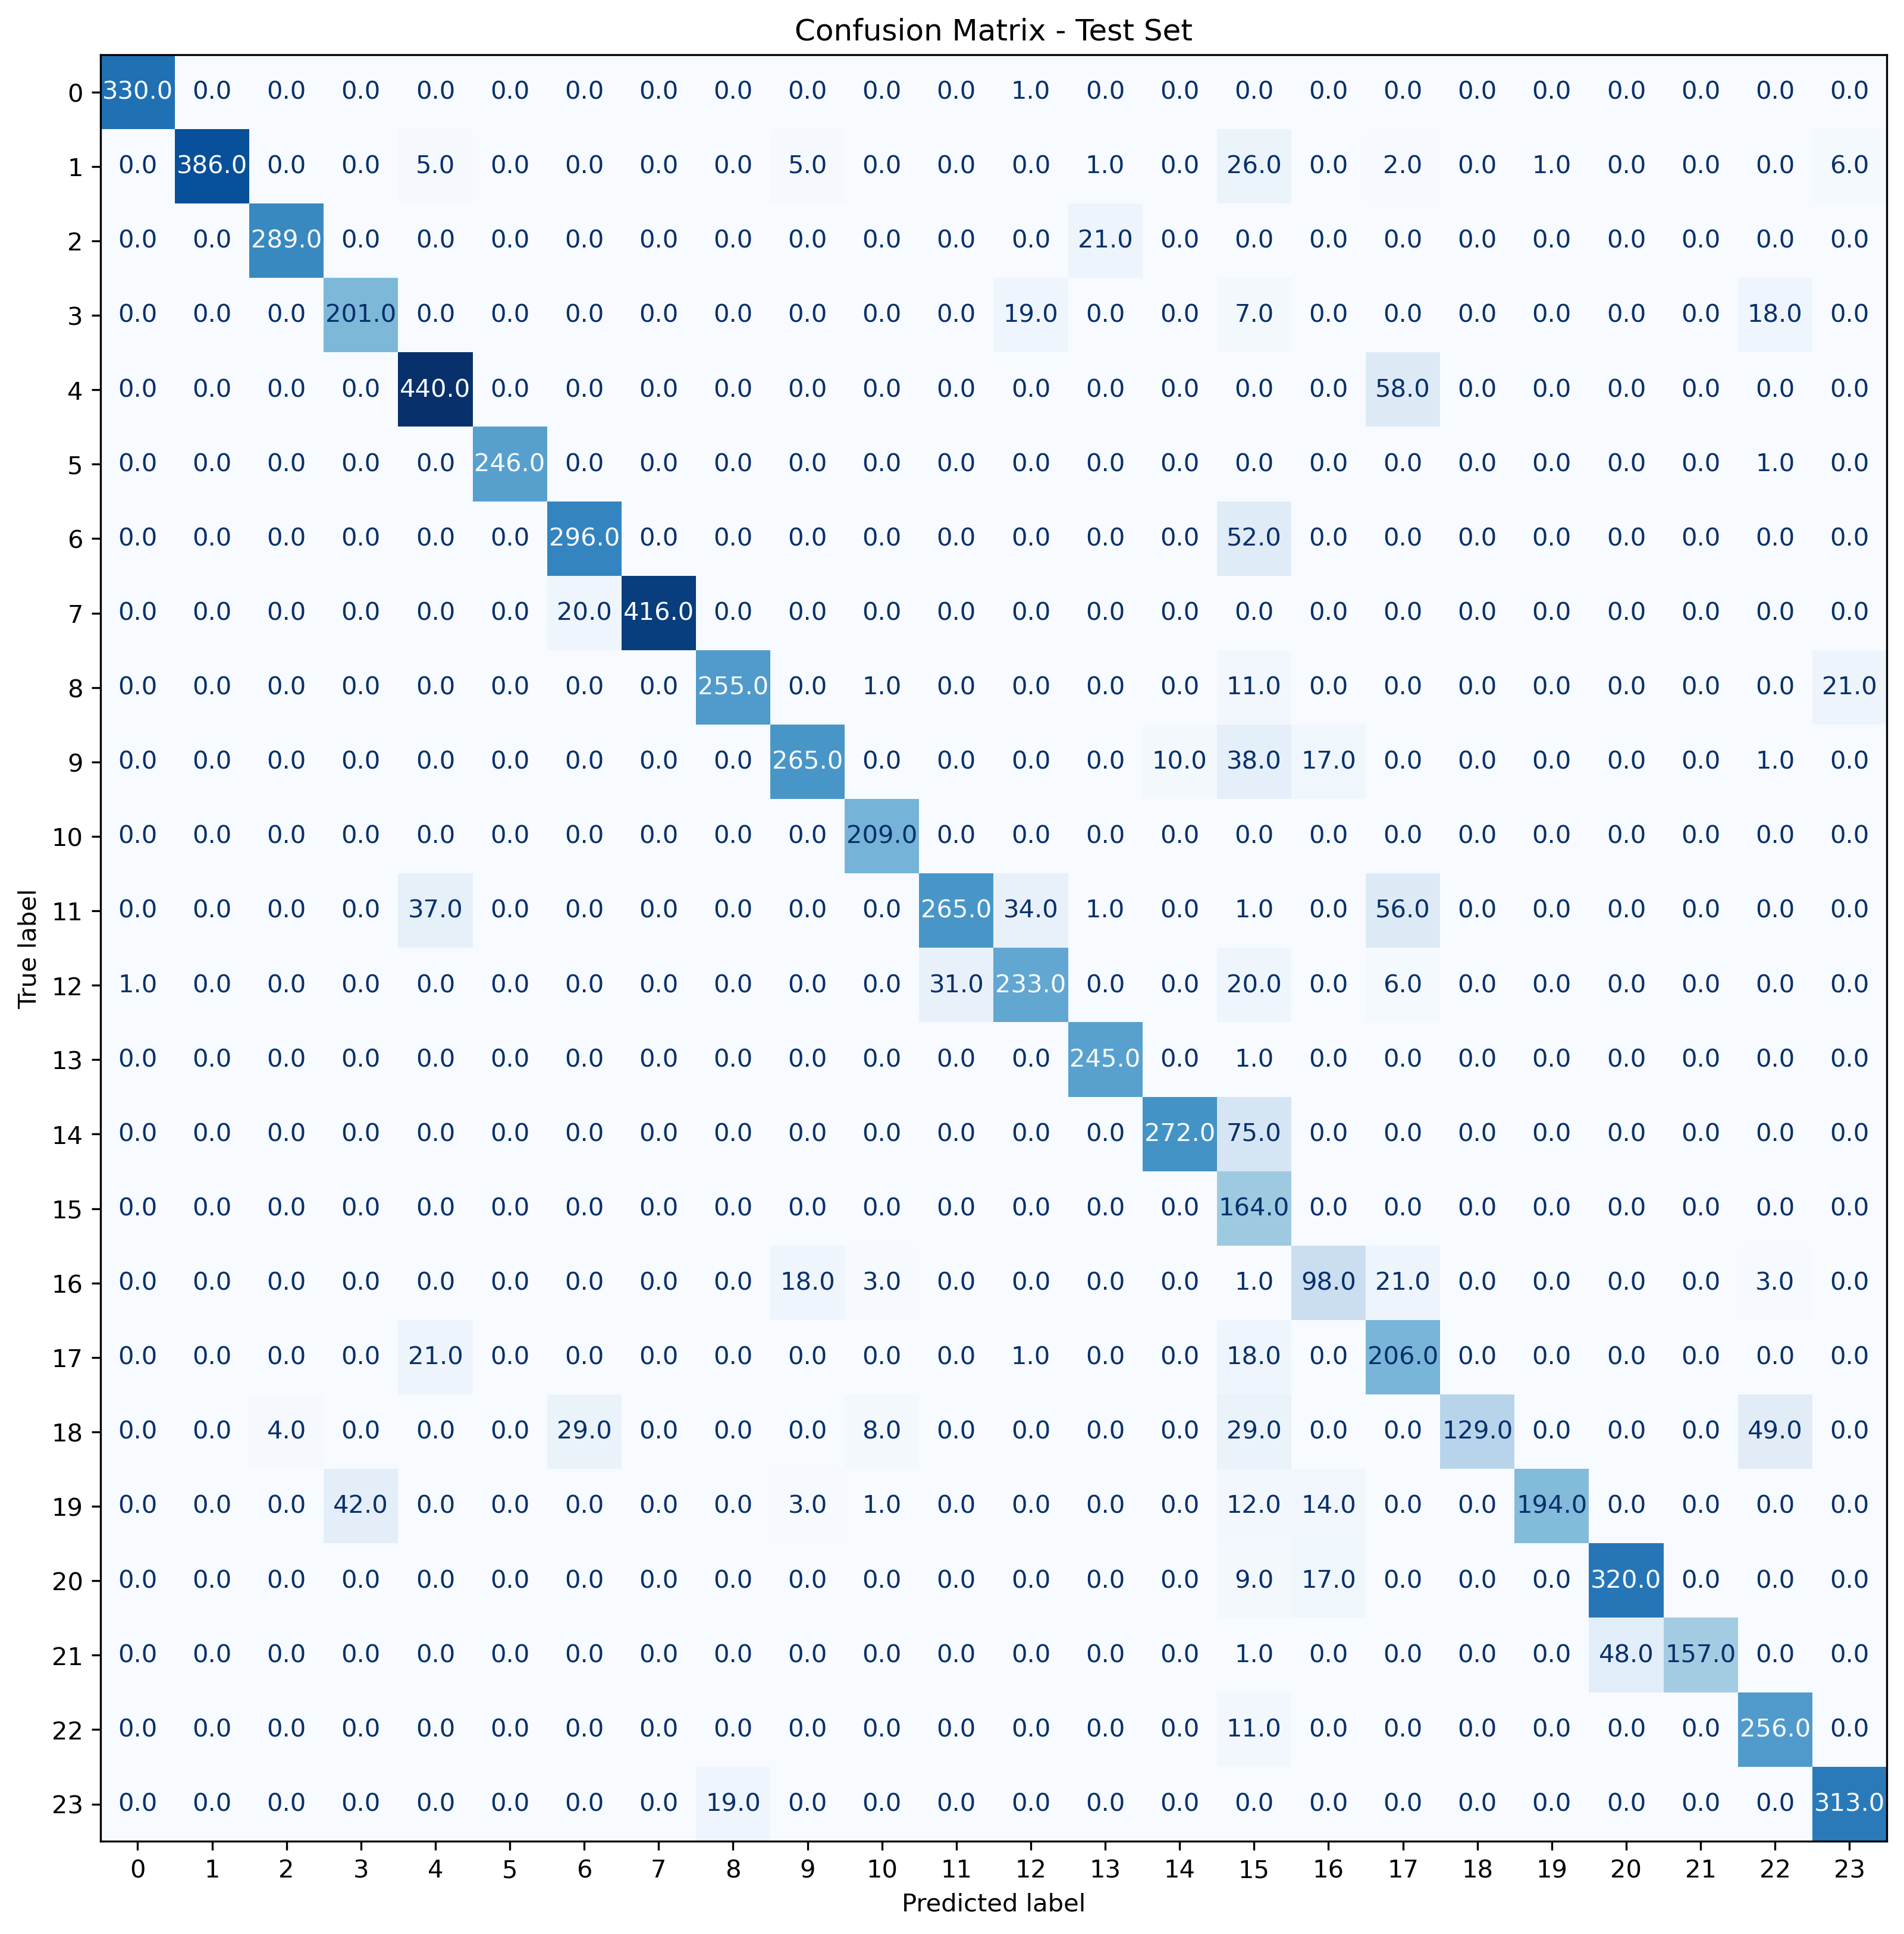
\includegraphics[width=0.5\linewidth]{../HW3_2/cnn1 cm.png}}
		\caption{ماتریس آشفتگی مدل \lr{CNN}}
		\label{fig:cnn1_cm}
	\end{figure}\\
	در این مدل برای جلوگیری از اورفیت شدن از لایه‌های \lr{Dropout} نیز استفاده شده است. یک نوع از این لایه‌ها که معمولا در شبکه‌های پیچشی موثرتر است لایه‌ی \lr{Block Dropout} می‌باشد. در حالت قبلی مقدار تعدادی از نورون‌ها به صورت تصادفی نادیده گرفته می‌شود که برای یک تصویر دو بعدی ممکن است هرجای شکل باشد. اما در لایه‌ی \lr{Block Dropout}، یک قسمت از تصویر پیکسل‌های آن مشابه هستند به صورت کامل، مثلا ۳ در ۳، نادیده گرفته می‌شوند. به این ترتیب به جای حذف شدن مقدار پیکسل‌ها به تنهایی، درواقع یک ویژگی از تصویر حذف می‌شود و در شبکه‌های پیچشی که ویژگی‌های مختلف از تصویر را استخراج می‌کنند مفید است.\\
	پیاده‌سازی این لایه به جای حالت قبلی، دقت را به $0.9541$ افزایش می‌دهد. نمودار خطا و دقت در
	\autoref{fig:cnn1}
و ماتریس آشفتگی در
\autopageref{fig:cnn2_cm}
آمده‌اند.\\
	\begin{figure}[!h]
		\centerline{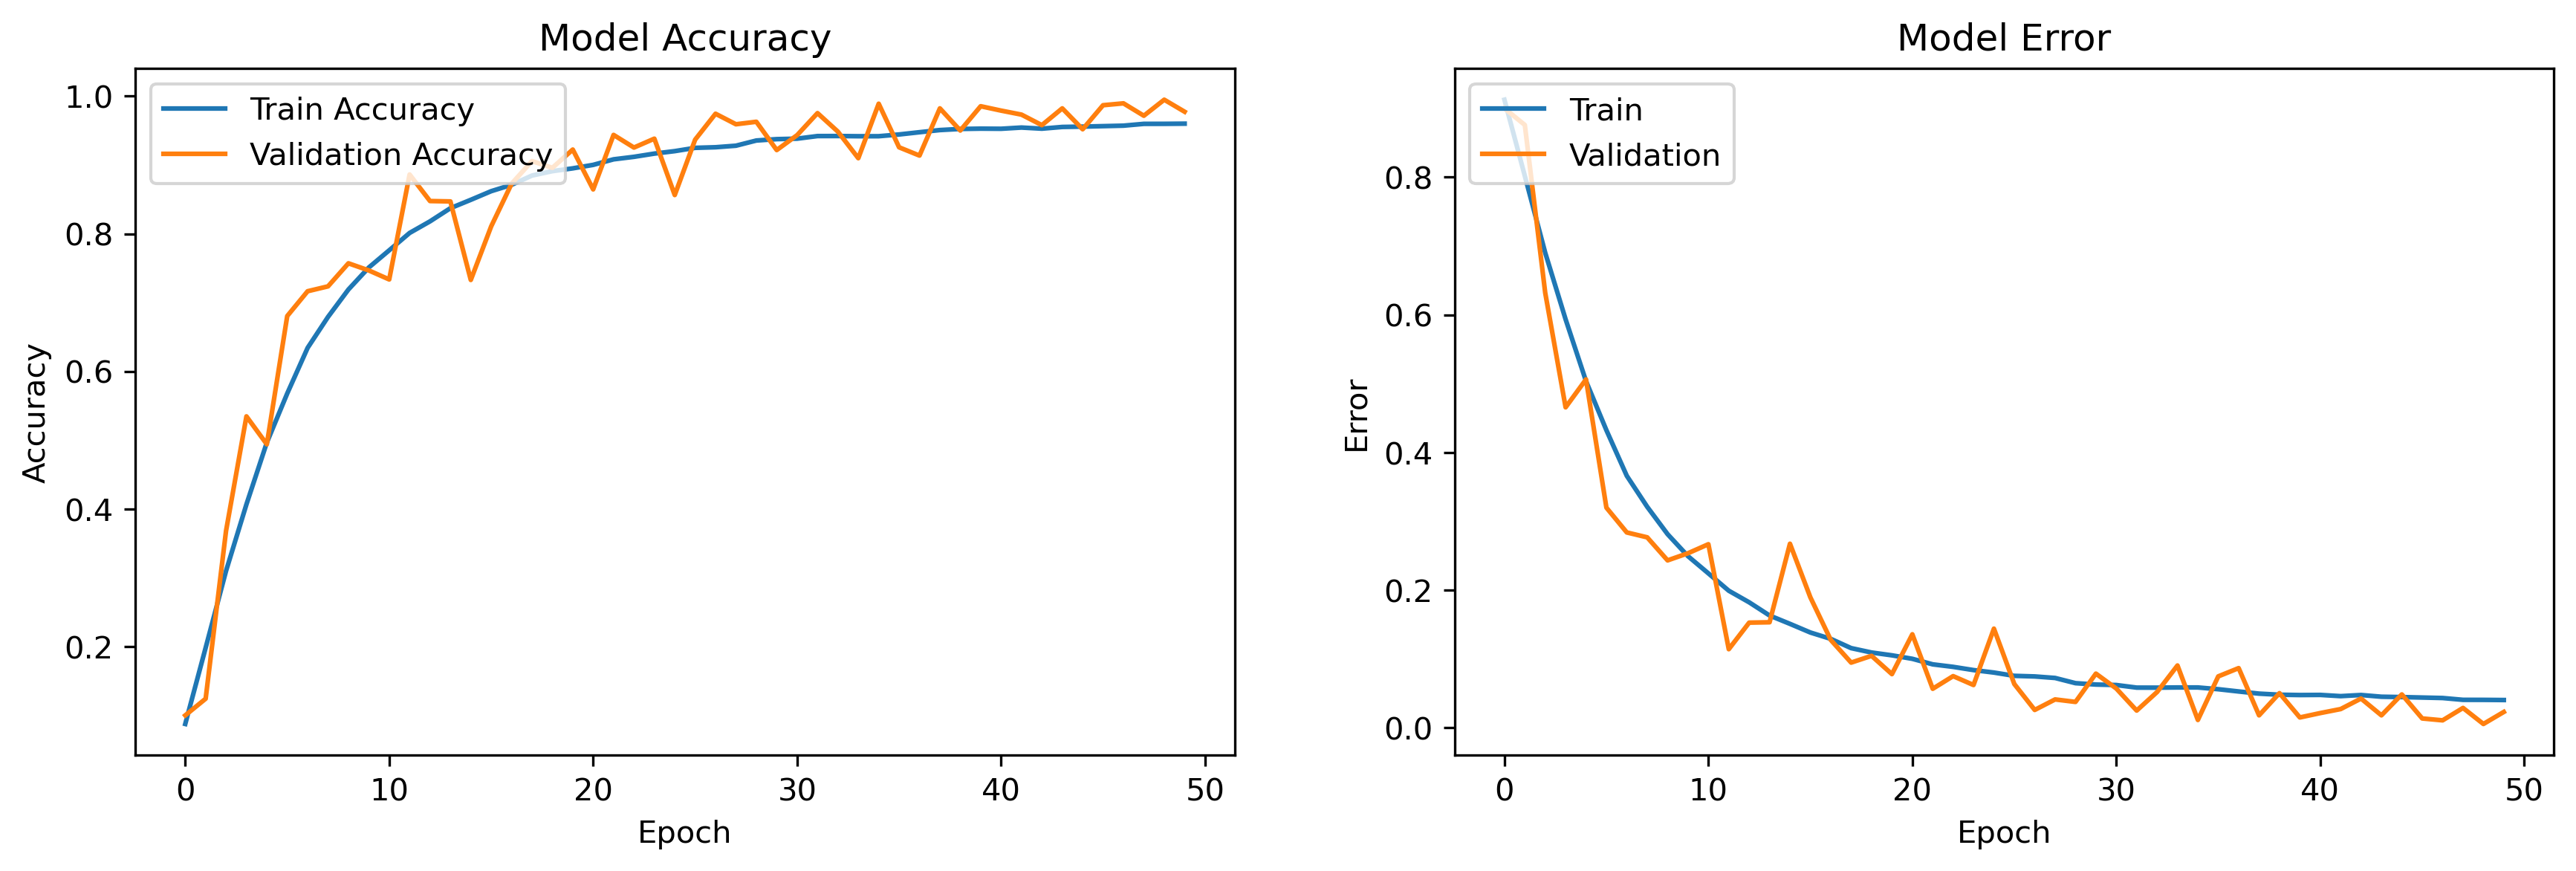
\includegraphics[width=1\linewidth]{../HW3_2/cnn2.png}}
		\caption{نمودار خطا و دقت  - مدل \lr{CNN} با \lr{Block Dropout}}
		\label{fig:cnn2}
	\end{figure}
	\begin{figure}[!h]
		\centerline{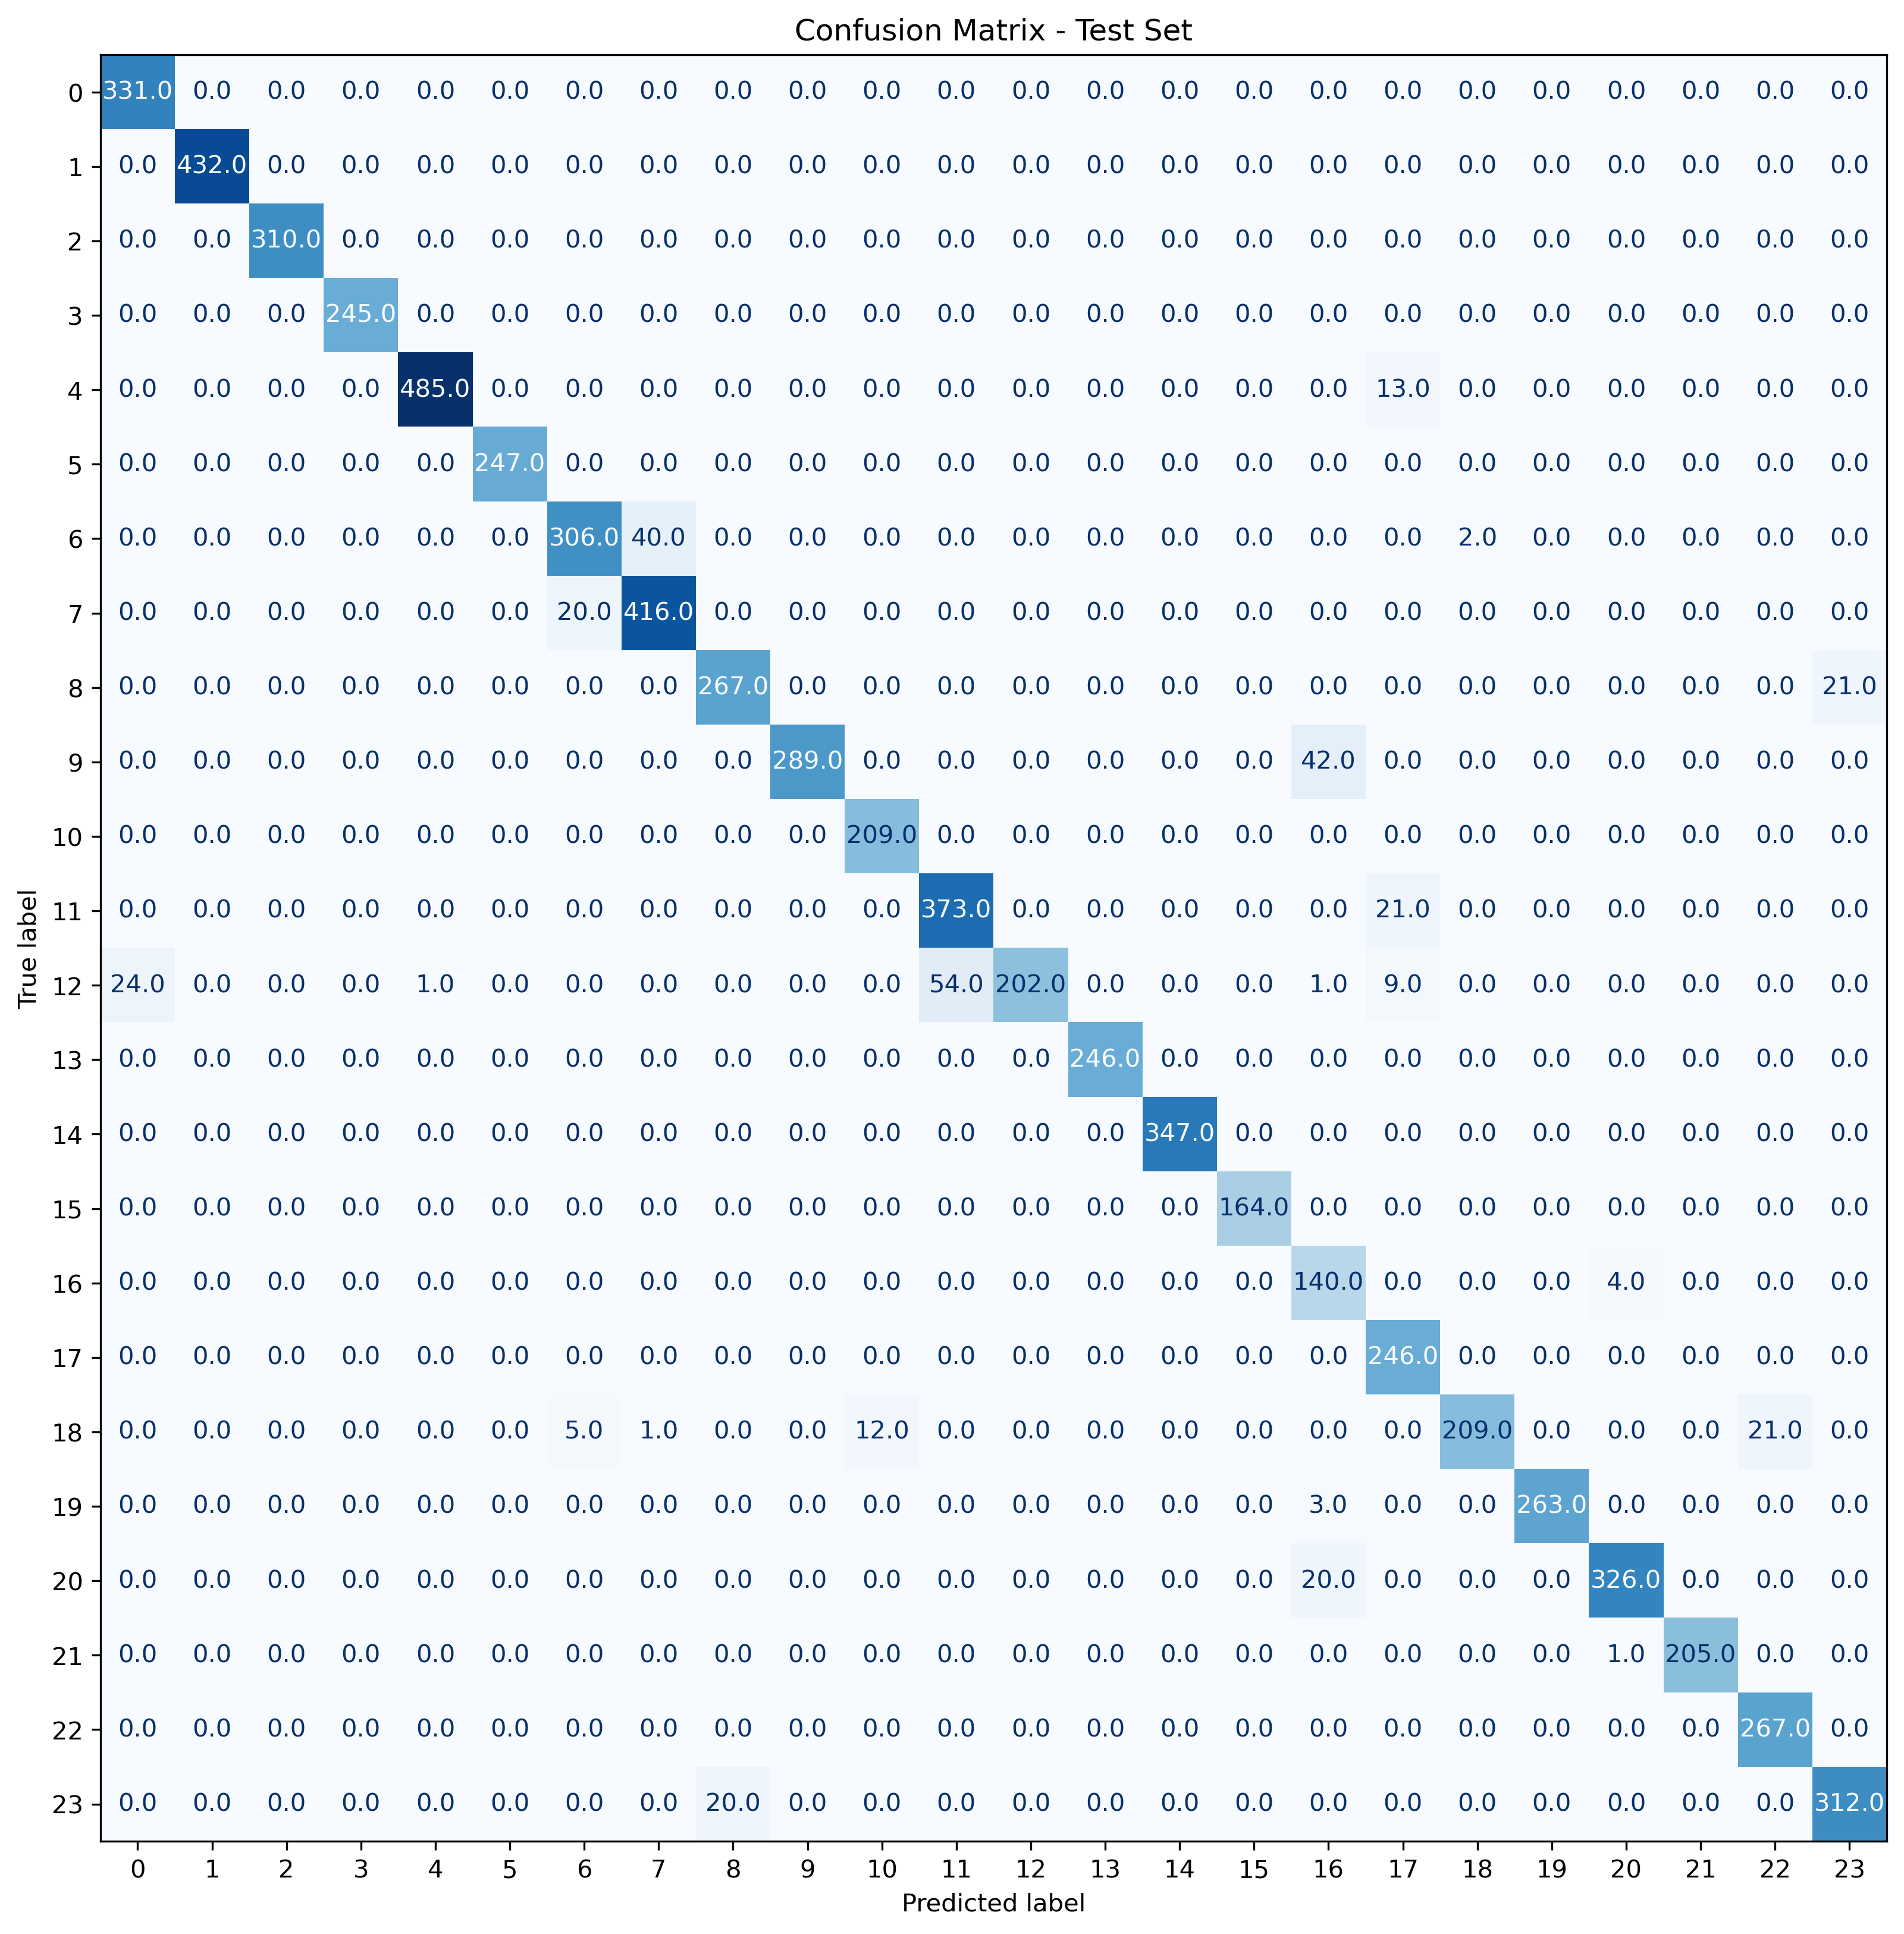
\includegraphics[width=0.5\linewidth]{../HW3_2/cnn2 cm.png}}
		\caption{ماتریس آشفتگی - مدل \lr{CNN} با \lr{Block Dropout}}
		\label{fig:cnn2_cm} 
	\end{figure}\\
	تجزیه فیلتر‌ها یا \lr{Kernel Factorization} روشی است که در آن فیلتر‌های لایه‌های پیچشی به فیلتر‌های کوچک‌تر تجزیه می‌شوند. به عنوان مثال یک فیلتر ۳ در ۳ به دو فیلتر ۱ در ۳ و ۳ در ۱ تجزیه می‌شود و در دو مرحله اجرا می‌شود. در همین مثال، در حالت اول ۹ پارامتر وجود دارند که باید تنظیم شوند ($ k^2 $) اما در حالت دوم ۶ پارامتر ($2k$) وجود دارد. بنابراین هنگام آموزش مدل هزینه محاسباتی پایین می‌آید. همچنین با کم شدن پارامتر‌ها، احتمال اورفیت شدن مدل نیز کاهش پیدا می‌کند. نتایج پیاده‌سازی این روش در
	\autoref{fig:cnn3}
	و
	\autopageref{fig:cnn3_cm}
	آمده‌اند. دقت نهایی این مدل روی داده‌های تست $0.9630$ می‌باشد.\\
		\begin{figure}[!h]
		\centerline{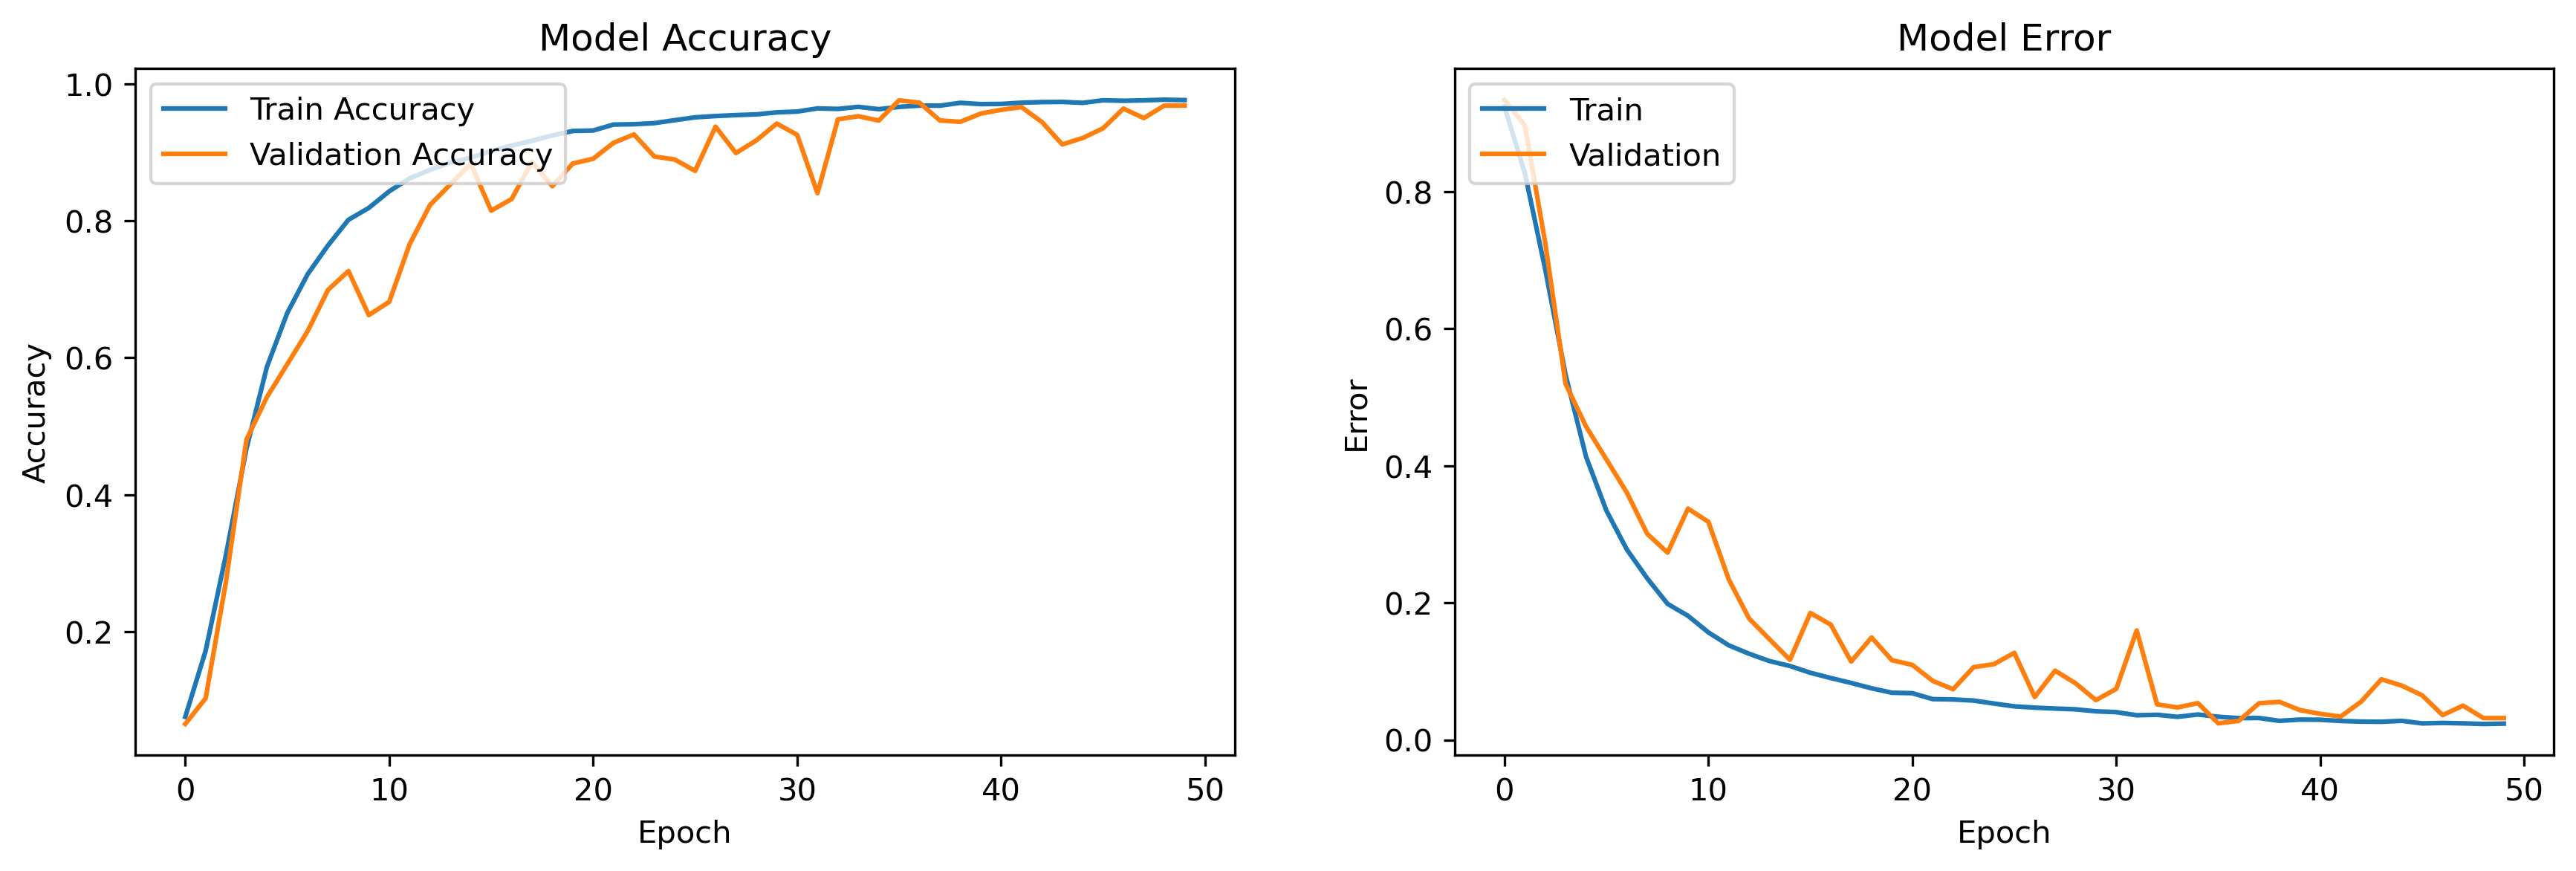
\includegraphics[width=1\linewidth]{../HW3_2/cnn3.png}}
		\caption{نمودار خطا و دقت  - مدل \lr{CNN} با تجزیه فیلتر‌ها}
		\label{fig:cnn3}
	\end{figure}
	\begin{figure}[!h]
		\centerline{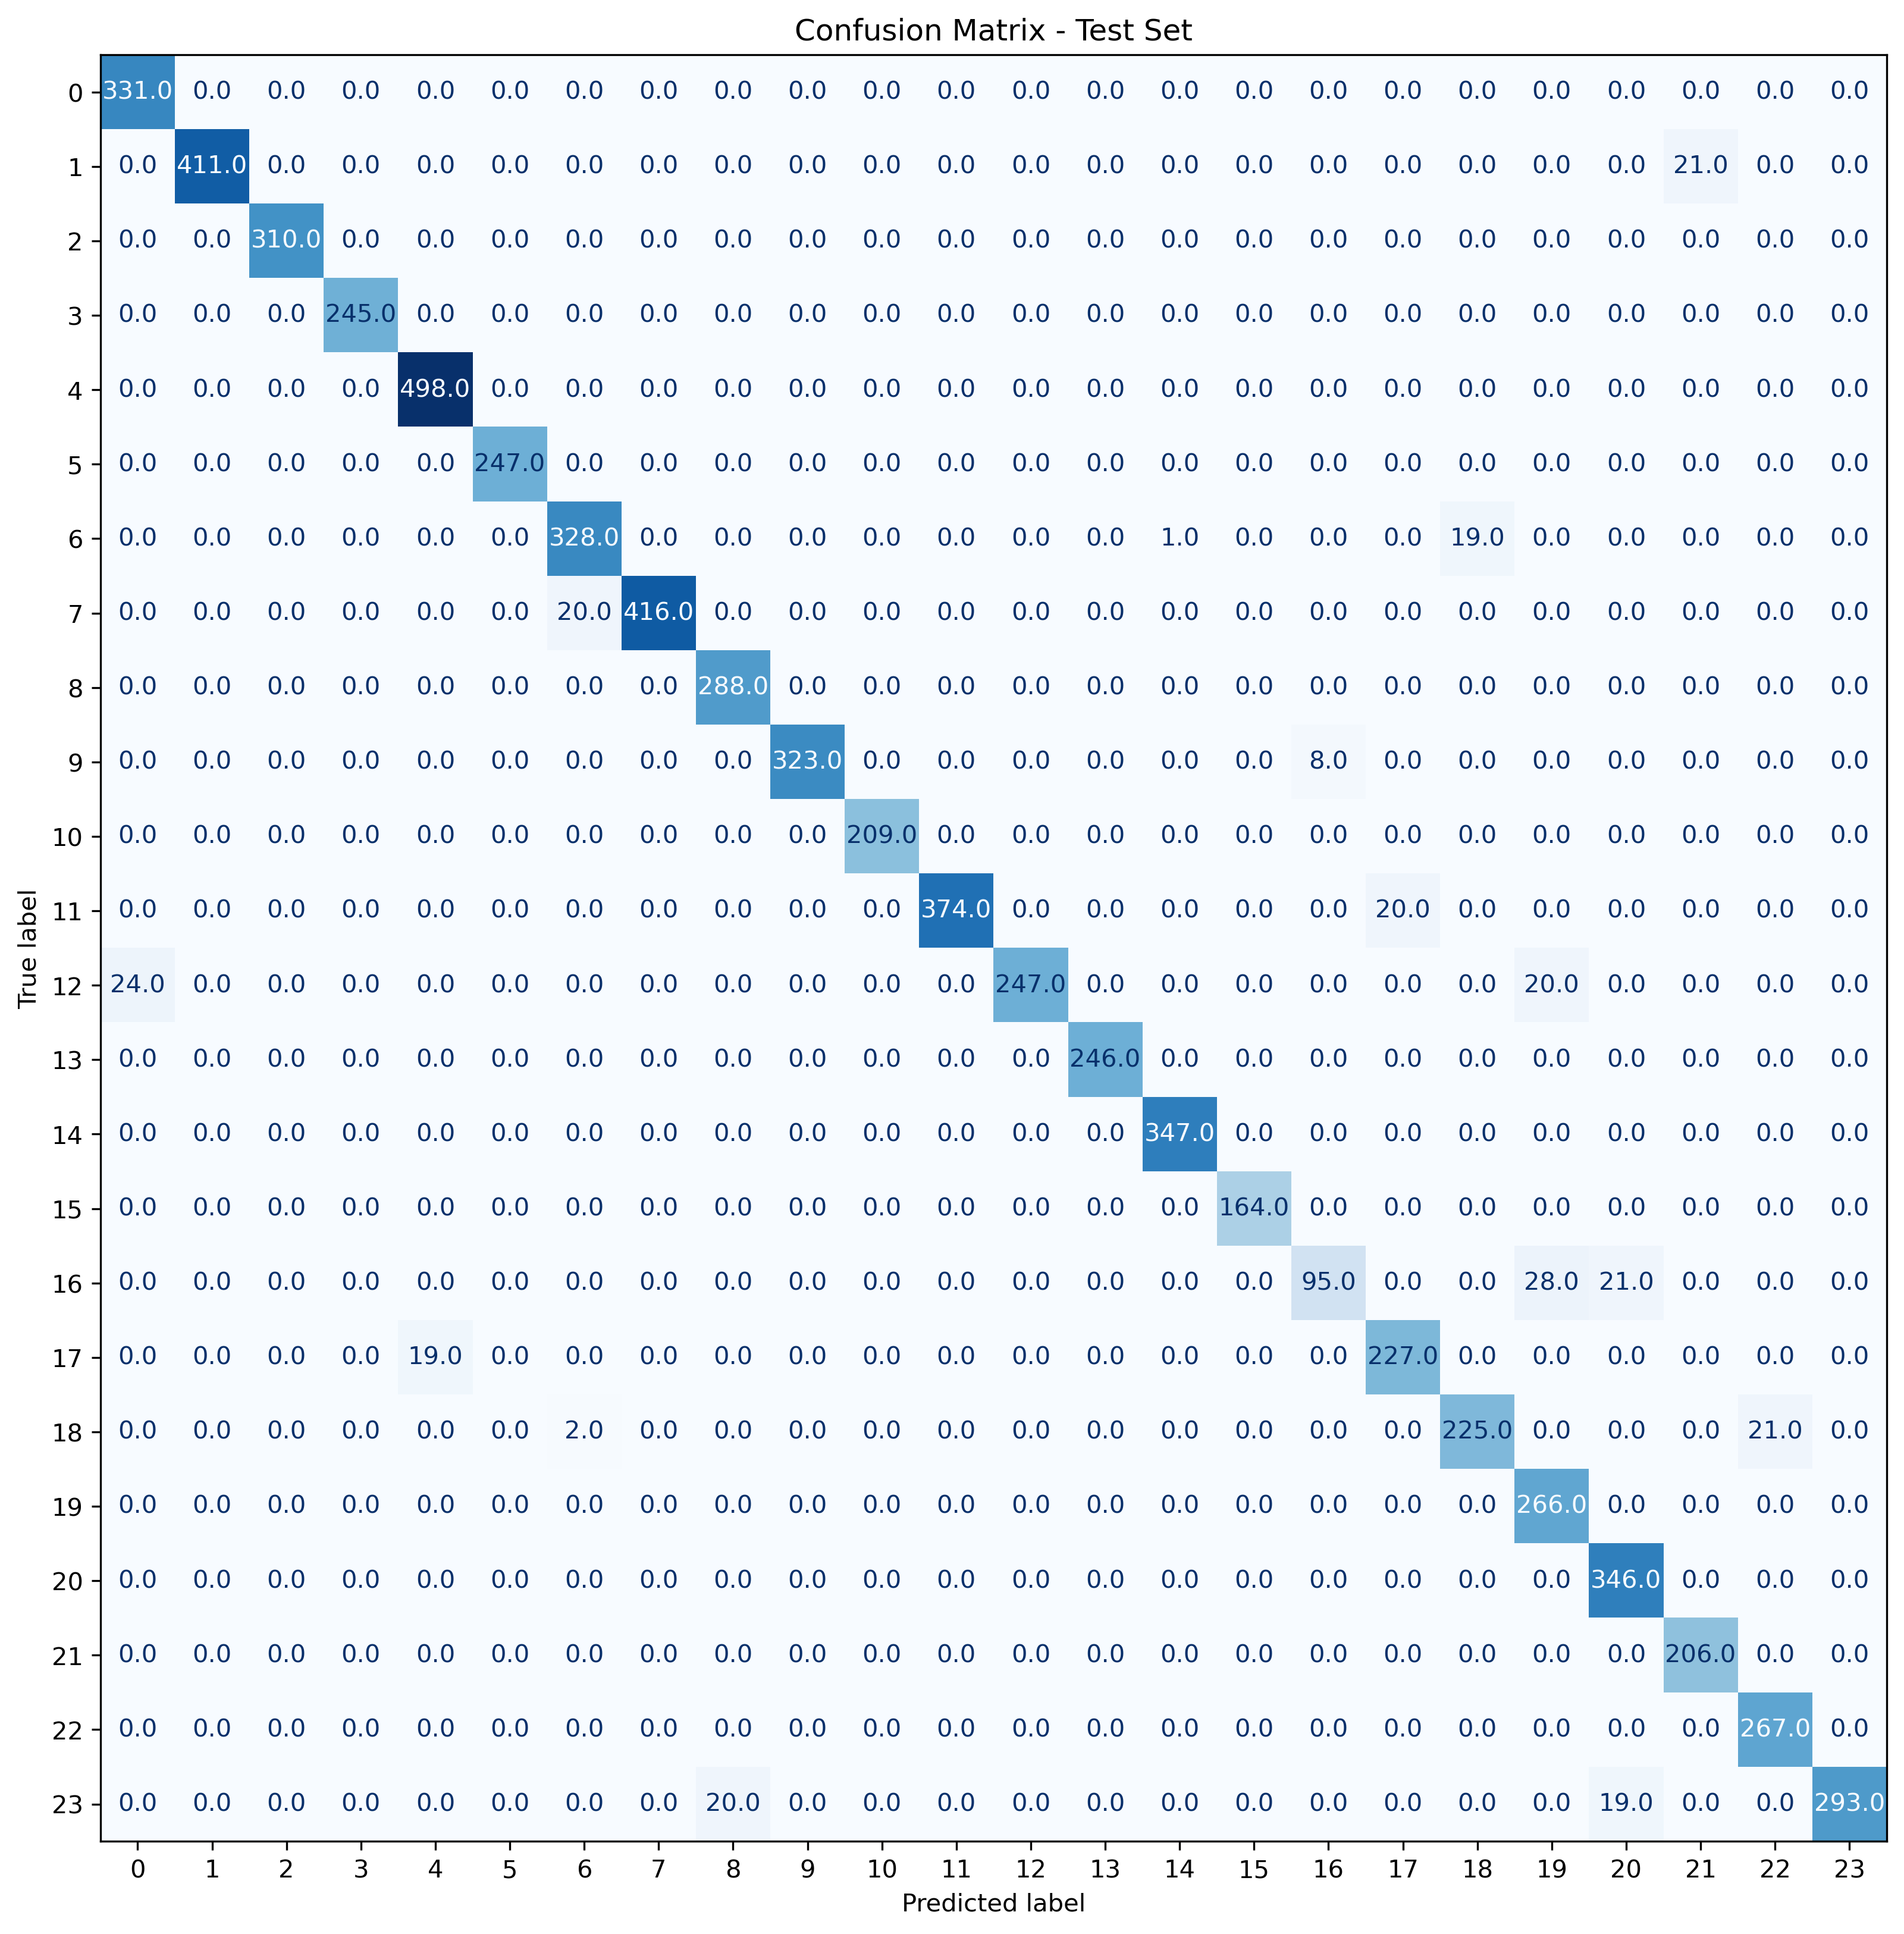
\includegraphics[width=0.5\linewidth]{../HW3_2/cnn3 cm.png}}
		\caption{ماتریس آشفتگی - مدل \lr{CNN} با تجزیه فیلتر‌ها}
		\label{fig:cnn3_cm} 
	\end{figure}\\
	در نهایت، جمع‌بندی دقت حالت‌های مختلف در 
	\autoref{tab:accuracy2}
	نوشته شده است.
		\begin{table}[h!]
		\caption{جمع‌بندی نتایج مدل‌ها برای پیش‌بینی دیابت}
		\begin{latin}
			\centering
			\begin{tabular}{|l|c|}
				\hline
				\textbf{Optimizer} &  \textbf{Test accuracy} \\ \hline
				CNN &  0.8599 \\ \hline
				CNN + Block Dropout &  0.9541 \\ \hline
				CNN + Kernal Factorization &  0.9630 \\ \hline
			\end{tabular}
		\end{latin}
		\label{tab:accuracy2} 
	\end{table}\\
	\section{آموزش انتقالی}
	در این قسمت باید ابتدا شبکه‌ای با ساختار \lr{ResNet50} با استفاده از داده‌های دیتاست \lr{EMNIST} پیش‌تربیت شوند و سپس با استفاده از همین مدل که ضرایب آن پیش‌تربیت شده‌اند، تربیت را با استفاده از داده‌های مسئله انجام داد. این کار نه تنها مواقعی که داده به اندازه کافی وجود ندارد به کار می‌آید، بلکه از جایی که از ضرایب پیش‌تربیت شده استفاده می‌شوند، روند تربیت دارای هزینه محاسباتی کمتری خواهد بود و سریع‌تر به دقت مورد نظر خواهد رسید. از همین رو تعدادی از این ضرایب از مدل‌های پیش‌تربیت شده مانند همین معماری شبکه در دسترس عموم بوده و می‌توان در مسائل استفاده کرد.\\
	داده‌های دیتاست \lr{EMNIST} مانند داده‌های مسئله عکس‌های تک کاناله ۲۸ در ۲۸ هستند که حاوی کاراکتر‌های مختلف دست‌نویسند. این دیتاست انواع مختلف دارد. در این مسئله از دیتاست \lr{Balanced} استفاده شده که در آن کل کلاس‌ها حاوی سمپل‌های یکسانی هستند. این دیتاست به صورت فایل \lr{.csv} در کد آپلود می‌شود.\\
	ورودی شبکه \lr{ResNet50} باید به اندازه $(n,n,3)$ باشد. به این معنی که تصویر مورد نظر باید دارای سه کانال باشد. همچنین حداقل اندازه تصاویر باید ۳۲ در ۳۲ باشند. به این ترتیب قبل از اینکه تصاویر دیتاست \lr{EMNIST} را بتوان به شبکه داد، باید اندازه آن را تغییر داد. این کار به کمک تابعی به نام 
	\verb|resize| 
	که در کد نوشته شده است انجام می‌شود. از جایی که هم شبکه پیچیده بوده و داده‌ها نیز زیاد هستند، این تابع عکس‌های تک کاناله ۲۸ در ۲۸ را گرفته و داده را به یک داده سه کاناله ۳۲ در ۳۲ تبدیل می‌کند تا کمترین محاسبات ممکن را داشته باشیم. لازم به ذکر است که سه کانال مورد نظر در تصویر نهایی دارای مقدار یکسان بوده و همان تک کانال تصویر اولیه هستند.\\
	سپس این تصاویر در بسته‌های دلخواه (در این کد ۳۲ تایی) با استفاده از کتابخانه 
	\verb|ImageDataGenerator|
	قرار داده می‌شوند تا به مدل داده شوند.
	\end{document} 